%#!platex jou.tex
\chapter{\LaTeX の基本}

\begin{abstract}
% commented out 2006/03/08
%まずは操作方法などの{\LaTeX}の基本を習得しましょう.本書ではあなたが
%\yo{何を書くべきか}ではなく\yo{どうやって書くべきか}ということしか説明
%しないことを始めに断っておきます,当たり前ですが.
まずは操作方法などの{\LaTeX}の基本を説明します.コンピュータの基本操作に
関する部分は大雑把にしか解説していませんので,適宜参考書を参照してくだ
さい.
\end{abstract}

\section{基本の基本}
\latexno{の基本}
\LaTeX は普通のワープロとは違い,ある程度の基本的な前提事項を踏まえなけ
ればなりません.ここでは\LaTeX を操作する上での基本の基本を解説します.


\subsection{処理の流れ}
\latexno{の動かし方}

%コマンドを覚える前にまずは{\LaTeX}での処理の流れを抑えておきましょう.テ
%キストファイルに文章そのものと\K{コマンド}というものを書き,それを
%\LaTeX 処理し,成形結果を確認するといったことを何度か繰り返して最終的な
%版を仕上げます\pp{\figref{latexflow}}.
\Z{コマンド}を覚える前にまずは{\LaTeX}での処理の流れをご覧下さい.
\Z{テキストファイル}に文章そのものと\KY{コマンド}というものを
書き,それを{\LaTeX}処理し,成形結果を確認するといった事を
何度か繰り返して最終的な\Z{版}を仕上げます\pp{\figref{latexflow}}.
\begin{figure}[htbp]
 \begin{center}
  \expandafter\ifx\csname graph\endcsname\relax \csname newbox\endcsname\graph\fi
\expandafter\ifx\csname graphtemp\endcsname\relax \csname newdimen\endcsname\graphtemp\fi
\setbox\graph=\vtop{\vskip 0pt\hbox{%
    \special{pn 8}%
    \special{pa 0 500}%
    \special{pa 750 500}%
    \special{pa 750 0}%
    \special{pa 0 0}%
    \special{pa 0 500}%
    \special{fp}%
    \graphtemp=.5ex\advance\graphtemp by 0.250in
    \rlap{\kern 0.375in\lower\graphtemp\hbox to 0pt{\hss 原稿の編集\hss}}%
    \special{pa 750 250}%
    \special{pa 1250 250}%
    \special{fp}%
    \special{sh 1.000}%
    \special{pa 1150 225}%
    \special{pa 1250 250}%
    \special{pa 1150 275}%
    \special{pa 1150 225}%
    \special{fp}%
    \graphtemp=\baselineskip\multiply\graphtemp by -1\divide\graphtemp by 2
    \advance\graphtemp by .5ex\advance\graphtemp by 0.250in
    \rlap{\kern 1.000in\lower\graphtemp\hbox to 0pt{\hss \MARU 1\hss}}%
    \special{pa 1250 500}%
    \special{pa 2000 500}%
    \special{pa 2000 0}%
    \special{pa 1250 0}%
    \special{pa 1250 500}%
    \special{fp}%
    \graphtemp=.5ex\advance\graphtemp by 0.250in
    \rlap{\kern 1.625in\lower\graphtemp\hbox to 0pt{\hss タイプセット\hss}}%
    \special{pa 2000 250}%
    \special{pa 2500 250}%
    \special{fp}%
    \special{sh 1.000}%
    \special{pa 2400 225}%
    \special{pa 2500 250}%
    \special{pa 2400 275}%
    \special{pa 2400 225}%
    \special{fp}%
    \graphtemp=\baselineskip\multiply\graphtemp by -1\divide\graphtemp by 2
    \advance\graphtemp by .5ex\advance\graphtemp by 0.250in
    \rlap{\kern 2.250in\lower\graphtemp\hbox to 0pt{\hss \MARU 2\hss}}%
    \special{pa 2500 500}%
    \special{pa 3250 500}%
    \special{pa 3250 0}%
    \special{pa 2500 0}%
    \special{pa 2500 500}%
    \special{fp}%
    \graphtemp=.5ex\advance\graphtemp by 0.250in
    \rlap{\kern 2.875in\lower\graphtemp\hbox to 0pt{\hss プレビュー\hss}}%
    \special{pa 3250 250}%
    \special{pa 3750 250}%
    \special{fp}%
    \special{sh 1.000}%
    \special{pa 3650 225}%
    \special{pa 3750 250}%
    \special{pa 3650 275}%
    \special{pa 3650 225}%
    \special{fp}%
    \graphtemp=\baselineskip\multiply\graphtemp by -1\divide\graphtemp by 2
    \advance\graphtemp by .5ex\advance\graphtemp by 0.250in
    \rlap{\kern 3.500in\lower\graphtemp\hbox to 0pt{\hss \MARU 3\hss}}%
    \special{pa 3750 500}%
    \special{pa 4500 500}%
    \special{pa 4500 0}%
    \special{pa 3750 0}%
    \special{pa 3750 500}%
    \special{fp}%
    \graphtemp=.5ex\advance\graphtemp by 0.250in
    \rlap{\kern 4.125in\lower\graphtemp\hbox to 0pt{\hss 出力・印刷\hss}}%
    \hbox{\vrule depth0.500in width0pt height 0pt}%
    \kern 4.500in
  }%
}%

  \usebox\graph
  \caption{処理の流れ}\figlab{latexflow}
 \end{center}
\end{figure}
ここで\yo{成形}とありますが,{\LaTeX}では元のソースファイルそのものに変
更を加えて\yo{整形}するのではなく,そこから新規に\Z{DVI}ファイルと
いうものを成形するのです \pp{最近は{\LaTeX}ファイルから直接PDFを作るプ
ログラム{\PDFLaTeX}なども存在します.\genzai 日本語化はされていませんが,
将来的には日本語を含む文書でも\PDFLaTeX が主流になると思われます}.

\index{原稿}%
\zindind{原稿}{の編集}%
\zindind{ソースファイル}{の編集}%
\index{編集}%
\indindz{編集}{原稿の}%
\indindz{編集}{ソースファイルの}%
\begin{enumerate}
\item 原稿\pp{ソースファイル}の編集\indindz{ファイル}{ソース}\\
{\LaTeX}を使うためには文章だけではなく,文章の構造や書式を決定する%
{\Z{コマンド}}と呼ばれるものを記述します. この原稿を\KY{ソースファイル}
と呼びます.原稿は\Prog{メモ帳}や\Z{Emacs}などの\Z{テキストエディッタ}で編
集します\pp{\laTEX は直接コンソールからプログラムを呼び出し,文書を執筆
する事も可能です}.\unixos では\Z{コンソール}から次のように入力するとEmacs
が立ち上がると思います.
\begin{InTerm}
   \type{emacs filename.tex &}
\end{InTerm}
Emacsでなくとも,お好きなテキストエディッタや,何らかの\secref{lakulaku}
にあるような執筆環境で良いと思います.これが\figref{latexflow}
の \MARU{1} の矢印に対応します.

\item タイプセット \pp{組版}\\
\latexno{の実行}%
ソースファイルができたらそれを\KY{成形}します.
そのときに使うプログラムは欧文のみの場合は\prog{latex},
日本語を扱うときは\prog{latex}を日本語化した{platex}です.
%シェルやコマンドプロンプトなどから
\Z{シェル}や\Z{コマンドプロンプト}などの\Z{ターミナル}から,
\begin{InTerm}
   \type{platex filename.tex}
\end{InTerm}
とすれば文書が成形されます.この作業の事を良く\KY{タイプセット}とか
\KY{コンパイル}と言います.これが\figref{latexflow}の \MARU{2} の矢
印に対応します.

\item プレビュー\pp{確認作業}\\
\indindz{文書}{組版後の}%
今度はコンピュータの画面上で成形された結果を見ます.
このとき\fl{filename.tex}そのものが整形されるわけではなく
新たに\fl{filename.dvi}というファイルが
作られます.これが{\LaTeX}による組版後の文書になります.この
組版後の結果をコンピュータ上で確認する作業の事を\KY{プレビュー}する
と言います.
Unix系OSならば
\begin{InTerm}
   \type{xdvi filename.dvi &}
\end{InTerm}
%commented out 2006/03/08
%などとすると良いでしょう.最後のアンパサンド\qu{\texttt{\&}}もあると便利です.
%\prog{dviout}をインストールしたWindowsならばダブルクリック
%するだけで見られるでしょう.これが\figref{latexflow}の
%\MARU{3}の矢印に対応します.
などとすると良いでしょう.最後のアンパサンド\qu{\texttt{\&}}があると
プログラムが\Z{バックグラウンド}で起動しますので便利です.
\prog{\Dviout}をインストールした\Z{Windows}ならば\Z{ダブルクリック}
するだけで見られるでしょう.これが\figref{latexflow}
の \MARU{3} の矢印に対応します.
\end{enumerate}
このような流れがある事を確認して実際に動くかどうかを試して
みましょう.

\subsection{動かしてみる}
インストールが済んでいれば{\LaTeX}が動きます.インストールまで
進んでいないという方は近くの詳しい方に聞いてみてください.
\yo{{\LaTeX}をやりたいんですが}と言い出せば大抵の{\LaTeX}ユーザは親切
に対応してくれると思います.

とりあえず自分のいつも使っているテキストエディッタ\pp{メモ帳やEmacs等}で
以下のようなファイル\Fl{test.tex}を作成してください%
\footnote{無用なトラブルを避けるため,ファイル名には半角英数の文字だけを
使い,可能な限り日本語は使わないようにしてください.}.Windows ユーザの
方はバックスラッシュ`\texttt{\bs}'を円記号`\texttt{\yen}'に読み替えてく
ださい.

\begin{InTeX}
\documentclass{jarticle}
\begin{document}
こんにちは \LaTeX !!
\end{document}
\end{InTeX}

\unixos ならば\prog{Emacs}等で良いでしょう.日本語を
打ち込むためには\prog{Emacs}の場合はまず\prog{Emacs}のウィンドウ下部に
注目してください.ウィンドウの下部の表示には
\begin{quote}
\colorbox{black}%
 {\color{white}\str{[--]J.:------Emacs: test.tex (LaTeX)--[L1--All--------|}}
\end{quote}
となっていると思います.
\index{入力}%
\indindz{入力}{半角}%
\indindz{入力}{英数}%
\indindz{入力}{全角}%
\indindz{入力}{日本語}%
一番右側の \colorbox{black}{\color{white}{\str{[--]}}} と
いう部分が半角入力\pp{英数入力}か全角入力\pp{日本語入力}かの違いを表します.
うえの状態は英数文字の入力ができます.ここで半角・全角の入力を切り替えるため
には\keytop{CTRL}を押しながら\keytop{\yen}を押します.すると
\colorbox{black}{\color{white}{\str{[--]}}}という表示から
\colorbox{black}{\color{white}{\str{[あ]}}}という表示になると思います.
表示は使っている\yo{\Z{かな漢字変換プログラム}}によって若干違うかもしれませ
ん\footnote{\key{Shift,Space}で切り替える場合もあります.}.
\colorbox{black}{\color{white}{\str{[あ]}}}の表示ですと日本語が入力
できる状態です.最近のパソコンと呼ばれるコンピュータには
\keytop{半角/全角}というキーがあり,Windowsの場合はそれで
半角と全角の切り替えを行いますが,Unix系OSは違いますので注意してくださ
い\footnote{比較的新しいと思われる \unixos であれば「全角/半角」入力の切
り替えが \keytop{半角/全角} キーでできる場合もあります.}.詳しくはご自
分のエディッタのマニュアルを見るなどの対応をしてください.


\zindind{Windows}{でのタイプセット}%
次はタイプセット作業\pp{{\LaTeX}処理,またはコンパイル}をします.
Windowsならば \win{スタート} メニューから \win{ファイル名を指定して実行} 
というメニューがあるので,そこに\yo{\str{command}}と入力して
\qu{OK}ボタンを押せばコマンドプロンプトが起動するはずです.
そしてシェル上やコマンドプロンプトでファイルが存在する
ディレクトリ\pp{Windowsの方はフォルダ}に移動して
\begin{InTerm}
   \type{platex test.tex}
\end{InTerm}
として{タイプセット}してください.するとコンソール\pp{端末}には
次のように表示されると思います.

\begin{OutTerm}
This is pTeX, Version 3.14159-p3.1.5 (euc) (Web2C 7.4.5)
(./test.tex
pLaTeX2e <2005/01/04>+0 (based on LaTeX2e <2001/06/01> patch level 0)
(/usr/local/share/texmf/ptex/platex/base/jarticle.cls
Document Class: jarticle 2002/04/09 v1.4 Standard pLaTeX class
(/usr/local/share/texmf/ptex/platex/base/jsize10.clo))
No file test.aux.
[1] (./test.aux) )
Output written on test.dvi (1 page, 236 bytes).
Transcript written on test.log.
\end{OutTerm}

始めに\Z{バージョン情報}を表示\footnote{実
は \TeX のバージョンは \Person{Donald}{Knuth} の思想により3.14159\ldots の様に
$\pi$ に収束するようになっています.}して終わりには\fl{test.dvi}に組版後
のファイルを出力し,処理状況を\fl{test.log}に書き出した事になっていま
す.\fl{test.tex}をタイプセットして出力された\fl{test.log}には
\Z{エラーメッセージ}などの重要な情報が書かれているときがあるので
何か問題が発生したときは眺めてみると良いでしょう.

\begin{Trick}
\laTEX がコンソールに表示するメッセージ(及び\Va{file}{log})には,
様々な情報が出力されます.丸括弧の後にファイル名があるような場合,
上記の例では \str{(./test.tex} というのは,ファイルが読み込まれている
階層を表しています.内容をもう少し分かりやすく書けば次のようになります.

\begin{InText}
 (./test.tex
   (/usr/local/share/texmf/ptex/platex/base/jarticle.cls
      (/usr/local/share/texmf/ptex/platex/base/jsize10.clo)
   )
   (./test.aux) 
 )
\end{InText}

\Exten*{aux}%
\fl{test.tex}が\fl{jarticle.cls}と\fl{test.aux}を子ファイル,
\fl{jarticle.cls}が\fl{jsize10.clo}を子ファイルとしてファイル読み込み
を行っている事が分かります.

各括弧と数字の場合,例えば`\str{[1]}'はページ番号を表しています.
コンソールに`\str{[}'のような表示で \LaTeX の処理が中断したとすれば,
あるページを組み上げている段階で何らかの問題に遭遇した事を意味します.
\end{Trick}

\zindind{タイプセット}{後の生成ファイル}
タイプセット後にはいくつかのファイルが生成されています.
コンソールから\prog{ls}\pp{Windowsの方は\prog{dir}}コマンドで
\begin{InTerm}
    \type{ls test.*}
\end{InTerm}
とすると,次の四つのファイルが存在する事を確認してください.

\begin{OutTerm}
test.aux test.dvi test.log test.tex
\end{OutTerm}

{\LaTeX}の原稿であるソースファイル\fl{test.tex}をタイプセットしただけで
三つもファイルが生成されました,%これは只事ではありません.
これらのファイルが一般的にどのような役割を持っているのかを説明します.
% commented out 2006/03/08
%\begin{description}
%\zindind{相互参照}{に必要なファイル}%
% \item[\fl{test.aux}] 次回のタイプセットに必要になる\K{中途ファイル}.
%    目次の作成や相互参照をするために必要なファイル.
% \item[\fl{test.dvi}] \fl{test.tex}をタイプセットして出来上がった
%    印刷できる\K{成形ファイル}.DVIファイルと呼ばれる.%
%	    \indindz{ファイル}{DVI}%
% \item[\fl{test.log}] \fl{test.tex}をタイプセットしたときの処理状況や
%    どのような流れで処理をしたのかが書いてある\K{ログファイル}.%
%	    \indindz{ファイル}{ログ}%
% \item[\fl{test.tex}] 先程作成した{\LaTeX}の原稿である%
%	    \K{ソースファイル}. 
%\end{description}
%\end{comment}
\begin{description}
 \item[\normalfont\Va{file}{aux}] 
  \latexno{の中途ファイル}%
  \zindind{相互参照}{に必要なファイル}%
  次回のタイプセットに必要になる\KY{中途ファイル}.
  目次の作成や相互参照をするために必要なファイル.

 \item[\normalfont\Va{file}{dvi}] 
  \zindind{印刷}{できるファイル}%
  \indindz{ファイル}{印刷できる}%
  \indindz{ファイル}{DVI}%
  \Va{file}{tex}をタイプセットして出来上がった\zindind{成形}{ファイル}%
  印刷できる\K{成形ファイル}.\Z{DVI}ファイルと呼ばれる.%

 \item[\normalfont\Va{file}{log}] 
  \latexno{のログファイル}%
  \indindz{ファイル}{ログ}%
  \latexno{処理状況}%
  \Va{file}{tex}をタイプセットしたときの処理状況や
  どのような流れで処理をしたのかが書いてある\KY{ログファイル}.%

 \item[\normalfont\Va{file}{tex}] 
  \latexno{原稿}%
  先程作成した{\LaTeX}の原稿である\KY{ソースファイル}. 
\end{description}



\subsection{原稿作成時の注意点}\seclab{chui}
\zindind{原稿}{作成時の注意}%
これまでの作業ができていれば数式や図表を含まない簡単な文書を
作成できる事でしょう.そして実際に長い文章を打ち込んでみて
ください.ただし10個の半角記号は特殊文字として{\LaTeX}に別の仕事をさせる
ために使いますのでそのまま使う事ができません.

\index{"#@\verb+#+}\glossary{"#@\verb+#+}%
\index{"$@\verb+$+}\glossary{"$@\verb+$+}%
\index{"&@\verb+&+}\glossary{"&@\verb+&+}%
\index{"\@\verb+\+}\glossary{"\@\verb+\+}%
\index{"^@\verb+^+}\glossary{"^@\verb+^+}%
\index{"_@\verb+_+}\glossary{"_@\verb+_+}%
\index{"{1"}@\protect\bgroup\verb+"{+"}}%
\glossary{"{1"}@\protect\bgroup\verb+"{+"}}%
\index{"{2"}@"{\verb+"}+\protect\egroup}%
\glossary{"{2"}@"{\verb+"}+\protect\egroup}%
\index{"~@\verb+~+}%
\glossary{"~@\verb+~+}%
\index{%@\verb+%+}%"
\glossary{%@\verb+%+}%"

\begin{quote}
\verb|# $ % & _ { } ~ ^ \ |
\end{quote}

さらに3個の記号は出力が違う文字記号になります.%"
\index{"|@\texttt{\symbol{'174}}}%"
\index{"<@\verb+<+}%"
\index{">@\verb+>+}%"
\begin{quote}
\str| \str< \str> はそれぞれ --- !` ?`
\end{quote}
となる事でしょう.
以上の13個の記号を文章中で出力するために面倒ですが,
バックスラッシュ\pp{円}記号を補ったり長い命令を打ち込みます.%''"

\glossary{"#@\hspace*{-1.2ex}\verb+"\#+}%"
\glossary{"_@\hspace*{-1.2ex}\verb+"\_+}%"
\glossary{"$@\hspace*{-1.2ex}\verb+"\$+}%"
\glossary{"%@\hspace*{-1.2ex}\verb+"\%+}%"
\glossary{"{1"}@\hspace*{-1.2ex}\protect\bgroup\verb+"\"{+"}}
\glossary{"{2"}@\hspace*{-1.2ex}"{\verb+"\"}+\protect\egroup}
\glossary{"&@"\hspace*{-1.2ex}"\verb+"\"&+}
%"
\index{ナンバー}%
\index{ドル}%
\index{パーセント}%
\index{アンパサンド}%
\index{波括弧}%
%"
%\begin{center}
% \begin{tabular}{cc|cc|cc|cc|cc|cc|cc|cc}
% \# & \verb|\#| & \$ & \verb|\$| & \% & \verb|\%| & \& & \verb|\&| &
% \_ & \verb|\_| & \{ & \verb|\{| & \} & \verb|\}| \\
% \end{tabular}
%\end{center}
\begin{InOut}
\# \$ \% \& \_ \{ \}
\end{InOut}
%
\C*{textasciitilde}\index{チルダ}%
\C*{textasciicircum}\index{ハット}%
\C*{textbackslash}\index{バックスラッシュ}%
\C*{textbar}\index{縦棒}%
\C*{textless}\index{小なり}%
\C*{textgreater}\index{大なり}%
\begin{InOut}
\textasciitilde  \textasciicircum  
\textbackslash   \textbar  
\textless        \textgreater
\end{InOut}
%\begin{center}
% \begin{tabular}{cc|cc|ccl}
% \T{textasciitilde} & \T{textasciicircum} & \T{textbackslash}\\
% \T{textbar}        & \T{textless}        & \T{textgreater}\\
% \end{tabular}
%\end{center}

\begin{Prob} 半角文字と全角文字を混在させてある程度の量の文章の
入力をしてください.特殊記号も含めるようにすると良いでしょう.
\end{Prob}


\subsection{フォルダ・ファイルの基本的な操作}

%ディレクトリの移動方法を知らない,フォルダの作り方を知らないという
%方のためにコマンドプロンプトやシェルでの主要なコマンドを紹介します.
%まずWindowsでは\tabref{Windowscommands}などの基本的なコマンドが
%提供されています.
\zindind{ディレクトリ}{の作り方}%
\zindind{フォルダ}{の作り方}%
\Z{ターミナル}上での\Z{ディレクトリ}の移動方法を知らない,
\Z{フォルダ}の作り方を知らないという方のために,
\Z{コマンドプロンプト}や\Z{シェル}での主要な\Z{コマンド}を紹介します.
\zindind{Windows}{でのファイル操作}%
まず{Windows}では\tabref{Windowscommands}などの基本的なコマンドが
提供されています.

\begin{wraptable}[12]{l}{19zw}
\zindind{フォルダ}{の新規作成}%
\zindind{フォルダ}{の移動}%
\zindind{ファイル}{の情報表示}%
\zindind{ファイル}{の名前の変更}%
\zindind{コマンド}{のヘルプの表示}%
 \caption{Windows OSの基本コマンド}\tablab{Windowscommands}
 \begin{tabular}{lll}
 \TR
 \Th{コマンド名} & \Th{意味}             \\ 
 \MR
 \Prog{mkdir} & 新規にフォルダを作成      \\
 \Prog{cd}    & ディレクトリを移動        \\
 \Prog{dir}   & ファイルの情報を表示      \\
 \Prog{move}  & ファイル名を変更したり移動\\
 \Prog{copy}  & ファイルをコピー          \\
 \Prog{del}   & ファイルを削除            \\
 \Prog{help}  & コマンドのヘルプを表示    \\ 
  \BR
 \end{tabular}
\end{wraptable}

それぞれのコマンドの使い方\pp{ヘルプ}は \type{mkdir /?} 等とする事で表示
できます.または \win{スタート} メニューの \win{ヘルプ} からコマンドプロ
ンプトについて調べてみても同様の事ができます.どちらかというとWindows
ヘルプを利用したほうが良いでしょう.

\latexno{の原稿執筆支援}%
\zindind{原稿}{の入力支援}%
コマンドプロンプトなどの操作に慣れていないという方は\secref{basic:lakulaku}を
参照して{\LaTeX}の\Z{入力支援}環境を使うのも良い方法です.

Unix系OSの方はコマンドを覚えなければ%仕事にならないでしょう.
操作に不便を感じると思われますので,日ごろから使うように習慣付けを
すると良いでしょう.
シェルと言っても何種類かありますし,シェルに関しては1冊の本になる
くらい奥の深いものなので詳細はそれらに譲ります.ここでは基本的な
ファイル操作のコマンドだけを\tabref{shcommands}に紹介します.
\indindz{ヘルプ}{簡易の}%
それぞれのコマンドの簡単なヘルプが見たいときは
\begin{InTerm}
   \type{mkdir --help | less}
\end{InTerm}
のようにすると\Prog{less}がページを整形します.\par
\begin{wraptable}[10]{r}{23zw}
\zindind{ディレクトリ}{の新規作成}%
\zindind{ディレクトリ}{の移動}%
\zindind{コマンド}{の情報表示}%
\indindz{コマンド}{内部}%
 \caption{Unix系OSの基本コマンド}\tablab{shcommands}
 \begin{tabular}{lll}  
  \TR
  \Th{コマンド名} & \Th{意味}            \\ 
  \MR
 \Prog{mkdir} & 新規にフォルダを作成      \\
 \Prog{cd}    & ディレクトリを移動        \\
 \Prog{ls}    & ファイルの情報を表示      \\
 \Prog{mv}    & ファイル名を変更したり移動\\
 \Prog{cp}    & ファイルをコピー          \\
 \Prog{rm}    & ファイルを削除            \\
 \Prog{help}  & 内部コマンドのヘルプを表示\\
 \Prog{man}   & コマンドのヘルプを表示    \\
 \BR
 \end{tabular}
\end{wraptable}
もう少し詳しいヘルプが見たいときは
\begin{InTerm}
   \type{man mkdir}
\end{InTerm}
とします.もっと詳しいヘルプが見たいときは
\begin{InTerm}
   \type{info mkdir}
\end{InTerm}
のようにすると\Prog{info}がページを整形します.
\prog{less}や\prog{info}の操作方法は若干癖がありますので慣れるまで
時間がかかるかもしれません.Unix系OSの基本的な操作方法,正規表現,
プロセス,ファイル・ディレクトリの概念などについては\appref{info}
の参考資料を参照してください.Unix系OSならば
\begin{InTerm}
   \type{emacs file.tex &}
   \type{platex file.tex}
   \type{xdvi file.dvi &}
\end{InTerm}
の三つの操作ができればなんとかなります.本書ではUnix系OSの
基本ツールなどまで詳しく解説しないのでご自分で調べてみてください.

\zindind{コマンド}{ラインオプション}%
コマンドに対してシェル上で一緒に渡す文字列の事を\KY{引数}
と呼びます.そして多くのコマンドは\K{{コマンドラインオプション}}
といってハイフン\qu{\str{-}}かハイフンが二つ\qu{\str-\str-}で始まる
引数を特別なスイッチとして扱います.このスイッチによってそのコマン
ドは挙動を変えます.それぞれのコマンドでどのようなコマンドラインオ
プションが使えるのかは各プログラムのヘルプを調べます.
\indindz{引数}{ハイフンで始まる}%

\begin{Prob} 以下の作業をコンソール上から行ってください.
Windowsの方は\prog{mv}を\prog{move}に,\prog{ls}を\prog{dir}
に,スラッシュ\qu{\str/}を円\qu{\texttt{\yen}}と置き換えてください.
\begin{InTerm}
  \type{echo message1 >> file.txt}
  \type{echo message2 >> file.txt}
  \type{mkdir anydir}
  \type{cd anydir}
  \type{mv ../file.txt ./}
  \type{ls}
  \type{more file.txt}
  \type{ls ../}
%\begin{comment}[2006/03/08 23:25:46]
%   \type{echo hogehoge \str>\str> hoge.txt}
%   \type{echo gehogeho \str>\str> hoge.txt}
%   \type{mkdir geho}
%   \type{cd geho}
%   \type{mv ../hoge.txt ./}
%   \type{ls}
%   \type{more ./hoge.txt}
%   \type{ls ../}
%\end{comment}
\end{InTerm} 
上記の操作はどのような結果をもたらしたと考えられるでしょうか.
%\begin{comment}[2006/03/08 23:25:46]
%新規にディレクトリ\fl{geho}を作成し,現在のディレクトリに
%存在していたファイル\fl{hoge.txt}を\fl{geho}ディレクトリに
%移動したと考えられるでしょう.最後の操作でうえの階層の
%ディレクトリに\fl{hoge.txt}がないことでそれを確認できます.
%\end{comment}
新規にディレクトリ\fl{anydir}を作成し,現在のディレクトリ%
\indindz{ディレクトリ}{カレント}%
(\Z{カレントディレクトリ})に存在していたファイル
\fl{file.txt}を\fl{anydir}ディレクトリに移動したと
考えられるでしょう.最後の操作でうえの階層のディレクトリ%
\indindz{ディレクトリ}{親}%
(\Z{親ディレクトリ})に\fl{file.txt}がない事でそれを確認できます.
\end{Prob}

\subsection{エラーに遭遇する}
\latexno{のエラー}%
{\LaTeX}処理をしていると\Z{エラー}に悩まされるかもしれません.{\LaTeX}
は文章中にコマンドなどに関するエラーを発見するとそこで処理を中断
します.処理を中断するとユーザにどうすれば良いかを促します.
このとき端末には\Z{疑問符}\qu{\str?}が表示されます.

% commented out 2005/xx/xx
%そうして,エラーに対してどの処理をすれば良いのかをユーザ
%に促すします.エラーを出さないコツは,一気に文
%書を書き上げるのではなく,こまめに{\LaTeX}処理を途中で実行すること
%です.こうすると,修正が容易になります.

%\qu{?}と表示されることが良くあります.これは文法上の誤りで,タイプミス
%などが考えられます.処理を強制終了するために,\keytop{X}を押してく
%ださい.それでもだめなときは\keytop{CTRL}を押しながら\keytop{C}か
%\keytop{D}を押してください.これで終了できます.間違いのある行番号
%を表示しますので,そのあたりで怪しそうな箇所を探します.たいていは
%括弧の数が足りないとか,スペルが間違っているなどの単純なものです.

\begin{Exe} まずは以下のソースファイル\Fl{errortest.tex}を作成し
てください.

\begin{InTeX}
\documentclass{jarticle}
\begin{document}
Hello & Goodbye! Give me $100! Give me 100%!
Under_bar is stranger. Is sharp sing #?
No its' \#. Hello \& Goodbye!! 
\end{document} 
\end{InTeX}

%次にこのファイルをタイプセットしてください.すると端末には
次に\fl{error.tex}を\type{platex error}でタイプセットしてください.
するとターミナルには次のように表示されるでしょう.
\index{Misplaced alignment tab character@\texttt{Misplaced alignment tab character \&}}%
\index{エラー!Misplaced alignment tab character@\texttt{Misplaced alignment tab character \&}}%

\begin{OutTerm}
! Misplaced alignment tab character  &.
1.3 Hello & 
            Goodbye! Give me $100! Give me 100%|
?
\end{OutTerm}

最後の行に疑問符\qu{\str?}が表示されています.この状態はユーザに何らかの
操作を促している状態です.どうやら3行目でアンパサンド\qu{\texttt\&}を不正に使っ
ていると言われています.ここで\keytop{Enter}キーを押すとさらに次のように
表示されます.

\index{You can't use `macro parameter character'@\texttt{You can't use
 `macro parameter character \#'}}%
\index{エラー!You can't use `macro parameter character@\texttt{You can't use
 `macro parameter character \#'}}%
\begin{OutTerm}
! You can't use `macro parameter character #' in math mode.
l.4 Under_bar is stranger. Is sharp sing #
? 
\end{OutTerm}

シャープ\qu{\texttt\#}も間違った使い方をしていると指摘されました.
極め付けにもう1度\keytop{Enter}キーを押すと次のような表示になります.%

\index{"$@\verb+$+}\glossary{"$@\verb+$+}%
\index{Missing $ inserted@\texttt{Missing \$ inserted}}%
\index{エラー!Missing $ inserted@\texttt{Missing \$ inserted}}%
\begin{OutTerm}
! Missing $ inserted.
<inserted text>
                $
l.6 \end{document}
? 
\end{OutTerm}

今度はドル\qu{\texttt\$}を
不正に使ったと言われました.以上の事から3行目から
6行目にかけて半角記号の使い方が間違っている事が分
かりました.ソースファイルをもう1度確認し,どこが
どう違うのかを判別し修正してください.

修正後のファイルは以下のようになるでしょう.

\begin{InTeX}
Hello \& Goodbye! Give me \$100! Give me 100%!
Under_bar is stranger. Is sharp sing \#?
No its' \#. Hello \& Goodbye!!  
\end{InTeX}

3行目のアンパサンド\qu{\texttt\&}とドル\qu{\texttt\$}と
4行目のシャープ\qu{\texttt\#}にバックスラッシュ\qu{\texttt{\bs}}を
付けます.これを再びタイプセットしてみてください.

\begin{OutTerm}
! Missing $ inserted.
<inserted text>  $
l.4 Under_
          bar is stranger. Is sharp sing \#?
? 
\end{OutTerm}

\zindind{改行}{された表示}%
今度はドル\qu{\texttt\$}の書き忘れがあると言われています.
4行目のエラーメッセージで丁度アンダーバー\qu{\texttt\_}
の部分で表示が改行されていますから,この部分に
間違いがある事が分かります.どうやらアンダーバーは
ドル\qu{\texttt\$}などと同じようにバックスラッシュが必要なようです.
ここでとりあえず\keytop{Enter}キーを押してタイプセットを
終了してください.一つ目のエラーが表示されます.

\begin{OutTerm}
! Missing $ inserted.
<inserted text>  $
l.6 \end{document}
?
\end{OutTerm}

タイプセットは中断しませんが,何か煩雑な表示が出現します.%$

\begin{OutTerm}
Overfull \hbox (152.35132pt too wide) in paragraph at lines 3--6
[]\OT1/cmr/m/n/10 Hello & Good-bye! Give me $100! Give me 
100Under$[]\OML/cmm/m/it/10 arisstranger:Issharpsing
\OT1/cmr/m/n/10 #?\OML/cmm/m/it/10 Noits[]\OT1/cmr/m/n/10 #
\OML/cmm/m/it/10 :Hello\OT1/cmr/m/n/10 &\OML/cmm/m/it/10 
Goodbye\OT1/cmr/m/n/10 !!$ 
\end{OutTerm}

% commented out 2006/03/08
%というごちゃごちゃした表示がでます.これは\dos{Overfull \bs hbox}
%という\K{警告}であることが分かります.次に成形後のDVIファイル
%\fl{errortest.dvi}をプレビューしてください.すると行がページ
%をはみ出しています.先程のアンダーバーに関するエラーにおいて
これは \dos{Overfull \bs hbox}
という\KY{警告}である事が分かります.次に成形後のDVIファイル
\fl{error.dvi}をプレビューしてください.すると行がページ
をはみ出しています.先程のアンダーバーに関するエラーにおいて
次のような表示がありました.

\begin{OutTerm}
<inserted text>  $
\end{OutTerm}

どうやら{\LaTeX}は自動的に%$
ドル\qu{\texttt\$}を挿入したようです.\qu{b}という文字が\qu{r}の
下付きの添え字になっています.さらに\qu{Give me 100Under$_b$}
となっており入力されたパーセント\qu{\texttt\%}と
感嘆符\qu{\texttt!}が出力されておらず,次の行の
\qu{Under}とくっついています.
% commented out 2006/03/08
%どうやら先程のごちゃごちゃ
%した警告はこの行がページをはみ出していることを言っている
%ようです.ですからファイル\fl{errortest.tex}はさらに次のよう
%に修正されます.
\indindz{警告}{煩雑な}%
どうやら先程の煩雑な警告はこの行がページをはみ出して
いる事を意味しているようです.
ですからファイル\Fl{errortest.tex}はさらに次のよう
に修正する事になります.

\begin{InTeX}
Hello \& Goodbye! Give me \$100! Give me 100\%!
Under\_bar is stranger. Is sharp sing \#?
No its' \#. Hello \& Goodbye!!   
\end{InTeX}

これで望み通りうまくいきそうです.実際に上記のファイルを
タイプセットし,その結果を吟味してください.
\end{Exe}

% commented out on 2006/03/08 
%{\LaTeX}の原稿をタイプセットしたときに端末に疑問符\qu{\str?}
%が表示されて処理が中断しますが,この段階でこちらも疑問符\qu{\str?}
%で返事を返すと
\zindind{処理}{の中断}%
{\LaTeX}の原稿をタイプセットしたときに端末に\Z{疑問符}\qu{\str?}
が表示されて処理が中断しますが,この段階でこちらも疑問符\qu{\str?}
で返事を返すと次のように表示されます.

\begin{OutTerm}
Type <return> to proceed, S to scroll future error messages,
R to run without stopping, Q to run quietly,
I to insert something, E to edit your file,
1 or ... or 9 to ignore the next 1 to 9 tokens of input,
H for help, X to quit.
? 
\end{OutTerm}

疑問符\qu{\str?}が表示されている段階で
上記に挙げるようなキーの入力をすると何らかの対処が
できるようです.
\begin{description}
 \item[\keytop{Enter}] 
   エラーに対して{\LaTeX}が適当な対処をした後にタイプ
   セットを続行します.
 \item[\keytop{S}] \keytop{Enter}キーを押し続けた
事と同じ動作をします.
 \item[\keytop{R}] エラーが検出されても停止せずに
ノンストップでタイプセットします. 
 \item[\keytop{Q}] \keytop{Q}を押した場合は
\KY{バッチモード}に入り処理が続きます. 
 \item[\keytop{I} \va{文字列}]  文字列を挿入してタイ
プセットを続けます.元の原稿に修正は加えられません.
 \item[\keytop{H}] そのエラーに対する英語のヘルプを
端末に表示します.
 \item[\keytop{X}] ゲームを終了します. 
\end{description}

\zindind{括弧}{の足りない状態}%
\keytop{X}キーは余り押してはいけません.括弧が足りない
というエラーの場合はとりあえず\keytop{Enter}キーを
押せばそのまま処理を続行できます.

タイプセットをしてアスタリスク\qu{\str{*}}が表示されて
処理が中断するときがあります.\keytop{Enter}キーを
押しても同じメッセージが表示されてどうにも
ならなくなります.\index{*@\verb+*+}%"

\begin{OutTerm}
*
(Please type a command or say `\end')
\end{OutTerm}

この場合コンソールから`\verb|\end{document}|'と入力して処
理が終了しなかった場合は強制的にプログラムを終了してください.ソース中で
何かミスをしていると思われます\footnote{慣れないうちはどこに記述間違いが
あるのかを見つけるのが難しいと思われますから,適当な場所に分かりやすいよ
うに\Z{ブレイクポイント}(タイプセットが停止する地点)を設けるのも手だと思い
ます.}.

\subsection{プレビューアの操作}
%commented out 2006/03/08
%プレビューを行うプログラムのことを\KY{プレビューア}と言います.
%OSによって使用可能なプレビューアが異なります.Windowsならば
%\Hito{大島}{利雄}の\Prog{dviout},\unixos ならば\Prog{xdvi},
%Red Hatならば\Prog{pxdvi}などを使い\fl{hoge.dvi}を各アプリケー
%ションで開きます.Windowsの場合は\prog{dviout}に関する豊富な
%ヘルプやマニュアルが用意されているのでそちらを読んでみてください.
%ここではUnix系OSで広く使われている\prog{xdvi}を例に操作方法を
%説明します.まずシェル上で\fl{hoge.dvi}の存在するディレクトリに
%移動し,\prog{xdvi}に対してファイル名を指定し,
\zindind{Windows}{のプレビューア}%
プレビューを行うプログラムの事を\KY{プレビューア}と言います.
OSによって使用可能なプレビューアが異なります.
\indindz{プレビュー}{Windowsでの}%
Windowsならば\Hito{大島}{利雄}の\Prog[dviout]{\Dviout},
\indindz{プレビュー}{Unix系OSでの}%
\unixos ならば\Prog{xdvi},
\indindz{プレビュー}{Red Hatでの}%
\Z{Red Hat}又は\Z{Fedora Core}ならば\Prog{pxdvi}などを使い
\Va{file}{dvi}を各アプリケーションで開きます.
Windowsの場合は\prog{\Dviout}に関する豊富なヘルプやマニュアルが
用意されているのでそちらを読んでみてください.
ここでは\unixos で広く使われている\prog{xdvi}を例に操作方法を
説明します.まずターミナル上で\Va{file}{dvi}の存在するディレクトリに
移動し,\prog{xdvi}に対してファイル名を指定し,
\begin{InTerm}
   \type{xdvi }\Va{file}{dvi} \str &
\end{InTerm}
のようにします.Unix系OSならばアンパサンド\qu{\texttt\&}をつけて
\KY{バックグラウンド}で起動します.%\pp{\figref{xdvisample}}
こうするとタイプセットを再度したときに自動的にDVIファイルを
再表示します.\Dviout でも同様の再表示機能があります.
%\begin{figure}[hbtp]
% \begin{center}
%  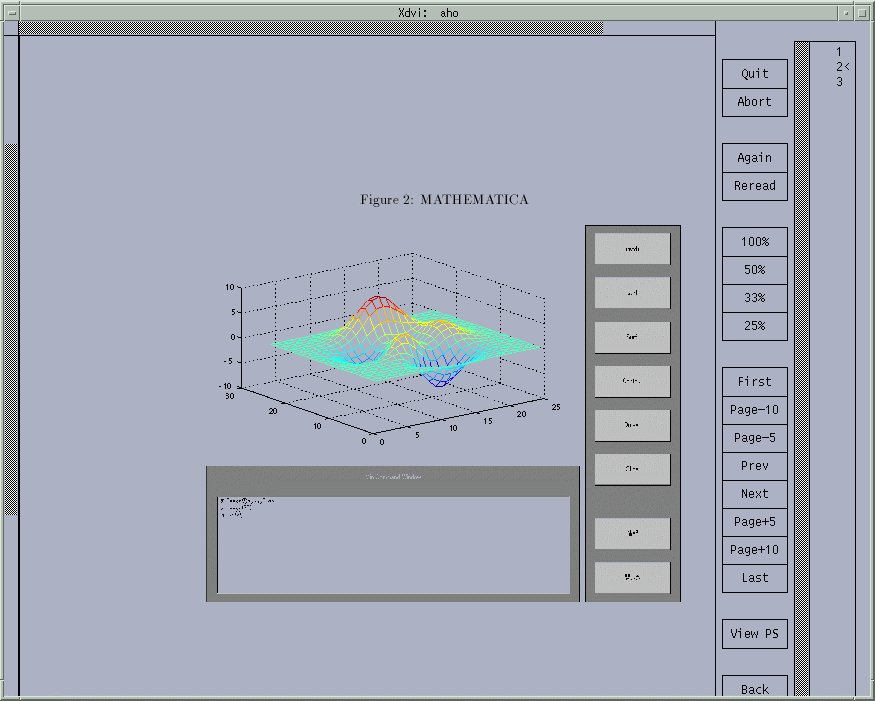
\includegraphics[bb={0 0 875 701},scale=.4]{images/xdvi}
%  \caption{{xdvi}の起動例}\figlab{xdvisample}
% \end{center}
%\end{figure}

\prog{xdvi}の基本的な操作方法を説明します.右側に枠で囲まれた
文字がボタンになっています.ボタンのように見えませんが一応押せます.
さらにボタンの右側にはページ番号があり,ページ番号をクリックすると
該当するページを表示します.

\prog{xdvi}でのマウスのクリックは拡大の機能を持っています.それぞれ
\begin{namelist}{中央クリック}
 \item[左クリック]   少し拡大.
 \item[中央クリック] 普通に拡大.
 \item[右クリック]   かなり拡大.
\end{namelist}
となっています.また,右側にある\qu{\str{Quit}}とか\qu{\str{Abort}}などは
ボタンで,主なボタンの機能は以下のとおりとです.
\begin{namelist}{View PS}
\item[\str{Quit}]
	    xdviを終了する.
\item[\str{Reread}]
	    一度読み込んだファイル\Va{file}{dvi}を再描画する.
\item[\str{First}]
	    先頭ページに移動する.
\item[\str{Prev}]
	    前ページに移動する.
\item[\str{Next}]
	    次ページに移動する.
\item[\str{Last}]
	    最終ページに移動する. 
\item[\str{View PS}]
	    {\PS}ファイルを見る.
\item[\str{File}]
	    DVIファイルを別に開く.
\end{namelist}

終了するには\qu{\str{Quit}}ボタンを押します. 


%\subsection{ちょっと休憩}
\begin{Trick}

これまで操作して少し疲れたでしょうから,ここで休憩をしましょう.
DVIファイルと言われてもなじみの薄いファイル形式かもしれません.
そこでこのDVIファイルを別のファイル形式に変換してみましょう.

例えば\PS に変換するには\pp{Windowsの方は\prog{dvipsk}}
\begin{InTerm}
  \type{dvips -o test.ps test.dvi}
\end{InTerm}
とすると\fl{test.dvi}から\fl{test.ps}が生成されます.この\fl{test.ps}を
\begin{InTerm}
  \type{ps2pdf test.ps test.pdf}
\end{InTerm}
としてPDFファイル\fl{test.pdf}を生成する事もできます.Postscript
ファイル\fl{test.ps}をプリンタに出力するには
\begin{InTerm}
  \type{lpr -P} \va{プリンタ名} \fl{test.ps}
\end{InTerm}
とする事で印刷要求を送信できます.\va{プリンタ名}については
システムの管理者に聞くなどしてください.

タイプセット時に拡張子\exten{tex}を省略して
\begin{InTerm}
  \type{platex test}
\end{InTerm}
としてみてください.以上のような例でも{\LaTeX}プログラムは
\fl{test.tex}を探し出してタイプセットしてくれるでしょう.

これは \LaTeX で使われているファイル検索の仕組みに関係しています.
\LaTeX では \Prog{Kpathsearch}というファイル検索機構を採用しています.
まず上記の例では\fl{test.tex}があるときに \type{platex test} とすると
\prog{Kpathsearch}が自動的に拡張子をつけてファイルを探します.
この時どのディレクトリ\pp{フォルダ}から探し出すかという情報が必要になりま
す.この情報が記載されたファイルは\Fl{texmf.cnf}というファイルです.
ほとんどの環境でディレクトリ \fl{\$texmf/web2c/} 以下にあります.%
\index{"$texmf@\texttt{\$texmf}}%
\index{ファイル!"$texmf@\texttt{\$texmf}}%
ここで \fl{\$texmf} は{\LaTeX}のファイルを格納すべき一番上のディレクトリを
示します.Unix系OSならば \fl{/usr/local/share/texmf/} 
などだったりWindowsならば \fl{C:\yen usr\yen local\yen share\yen 
texmf\yen} だったりするでしょう.
\begin{InTerm}
  \type{kpsewhich texmf.cnf}
\end{InTerm}
とすると,どこに\fl{texmf.cnf}が存在するのかが分かります.
\end{Trick}

\begin{Trick}
最近の \LaTeX プログラムは\prog{Kpathsearch}に対応しているので
何も意識しなくても適切に設定ファイルやクラスファイルなどを検索
してくれます.しかし手動で検索したいときもあると思います.
このような場合は\Prog{kpsewhich}というプログラムを使って
  \type{less `kpsewhich  book.cls`}
とすると\Fl{book.cls}というファイルが\fl{\$texmf}以下の
特定のディレクトリから検索され,\Prog{less}がファイルを
整形します.実はKpathsearch ではプログラム毎にファイルを
検索する場所を指定できます.そのため,\Fl{jarticle.cls}
というファイルを\type{kpsewhich jarticle.cls}としただけで
は検索結果に表示されません.\copt{-progname}というコマンドライン
オプションを付けて\type{kpsewhich -progname=platex jarticle.cls}
と実行すると,\pLaTeX が \Fl{jarticle.cls} というファイルを
見つけられる事になります.これにより複数のプログラムで同じ名前のファイル
名が存在しても,ディレクトリを変えておけば衝突しませんし,ファイルを検索
するディレクトリが少なくて済みますので処理速度が向上します.
\end{Trick}



\subsection{コマンド}

\zindind{原稿}{の構成}%
\zindind{原稿}{の先頭部分}%
{\LaTeX}では原稿を三つのパートに分割する事ができます.
それに伴いいくつかのコマンドは,特定のパートでしか使用
できません.
\begin{Syntax}
\verb|原稿先頭部分 (イニシャルコマンドを記述)|\\
\cmd{documentclass}\opa{オプション,$\ldots$}%
	\pa{クラス}\opa{リリース}\\
\va{前書き部分} (プリアンブルコマンドを記述)\\
\verb|\begin{document}|\\
\va{本文} (ボディ)\\
\verb|\end{document}|
\end{Syntax}
この中で \Cmd{documentclass},\Env{document}環境は必須であり,
絶対に必要な記述です.

\indindz{コマンド}{イニシャル}\indindz{コマンド}{プリアンブル}%
\zindind{プリアンブル}{コマンド}%
原稿先頭\pp{イニシャル}部分には\KY{イニシャルコマンド}と
呼ばれるコマンドを記述する事ができ,
同じように前書き\pp{プリアンブル}部分には%
\K{プリアンブルコマンド}や定義などを
記述する事ができます.そして,\env{document}環境
によって挟まれた本文部分にはコマンドの定義や組版用のコマンドを
記述します.それぞれのコマンドは定められた場所で使うように
決められています.ユーザがプリアンブルコマンドを本文で使う事が
できないように{\LaTeX}の内部で細工が施されています.

ここで言葉の定義をしましょう.コマンド,命令,環境,引数,オプションなど
の言葉を混同しがちですが,\K{本書では}以下のように取り決めます
\footnote{コマンドについての説明としては不十分なのですが,今は命令と環境
があると解釈してください.}.

\begin{description}%{コマンド}
\item[\Z{コマンド}] 
  \indindz{記号}{円}%
   \Z{バックスラッシュ}%
   \pp{Windowsの方は\Z{円記号}}と共に用いられる文字列.
   \begin{description}%{命令}
    \item[\Z{命令}]
       単独で使用するコマンド.
       引数を取る事ができる.
    \begin{quote}例:\verb|\alpha|,\verb|\maketitle|
          \end{quote}
    \item[\Z{環境}] 
       \qu{\C{begin}\pa{何々}}と
       \qu{\C{end}\pa{何々}}で囲まれている
     領域,またはそれを囲むためのコマンド.
       引数を取ることができる.
     \begin{quote}例:\verb|\begin{center}| \va{文字列} \verb|\end{center}|
    \end{quote}
   \end{description}
 \item[\Z{引数}] 
\zindind{コマンド}{の引数}%
\indindz{引数}{コマンドの}%
   コマンドに受け渡す文字列.
   \begin{description}%{必須引数}
    \item[\Z{必須引数}] 
\indindz{引数}{波括弧で挟まれた}%
\indindz{引数}{必須の}%
\zindind{波括弧}{で囲まれた引数}%
\zindind{波括弧}{の役割}%
       {波括弧}\qu{\texttt{\char'173~\char'175}}で囲まれた要素.
       コマンドが必須引数を取るときは必ず受け渡す.
           \begin{quote}例:\verb|\section|\pa{見出し語}\end{quote}
   \item[\Z{任意引数}] 
\indindz{引数}{角括弧で挟まれた}%
\indindz{引数}{任意の}%
\zindind{角括弧}{で囲まれた引数}%
       オプションとも言う.\Z{角括弧}\qu{\texttt{[~]}}で囲まれた要素.
       コマンドが任意引数を取るときは任意に受け渡す.
          \begin{quote}例:\verb|\documentclass|\opa{任意引数}\pa{クラス名}
    \end{quote}
   \end{description}
\end{description}
% commented out 2006/03/09 
%\begin{description}%{コマンド}
%\item[\Z{コマンド}] 
%	   \Z{バックスラッシュ}%
%	   \pp{Windowsの方は\Z{円記号}}と共に用いられる文字列.
%	   \begin{description}%{命令}
%	    \item[\Z{命令}]
%		       単独で使用するコマンド.
%		       引数を取ることができる.
%	    \begin{quote}例:\verb|\alpha|,\verb|\maketitle|
%            \end{quote}
%	    \item[\Z{環境}] 
%		       \qu{\Cmd{begin}\pa{なんとか}}と
%		       \qu{\Cmd{end}\pa{なんとか}}で囲まれている
%		       領域,またはそれを囲むためのコマンド.
%		       引数を取ることができる.
%            \begin{quote}例:\verb|\begin{center}文字列\end{center}|
%	    \end{quote}
%	   \end{description}
% \item[\Z{引数}] 
%	   コマンドに受け渡す文字列.
%	   \begin{description}%{必須引数}
%	    \item[\Z{必須引数}] 
%		       波括弧\qu{\texttt{\{\}}}で囲まれた要素.
%		       コマンドが必須引数をとるときは必ず受け渡す.
%            \begin{quote}例:\verb|\section{引数}|\end{quote}
%	    \item[\Z{任意引数}] 
%		       オプションとも言う.角括弧\qu{\texttt{[]}}で囲まれた要素.
%		       コマンドが任意引数をとるときは任意に受け渡す.
%            \begin{quote}例:\verb|\documentclass[任意引数]{jbook}|
%	    \end{quote}
%	   \end{description}
%\end{description}


\subsection{括弧について}

%さて,{\LaTeX}の基本を知った所で\KY{括弧}に
%ついての取決めをしたいと思います.括弧については色々な呼
%び方があるようですが,誤解を避けるために\K{本書では}
%以下のように定義します.
%\begin{description}
% \item[\Z{かぎ括弧} \qu{「」}] 
%	    引用や会話文などに使う.
% \item[\Z{2重かぎ括弧} \qu{『』}] 
%	    書名,引用の中の引用などに使う.
% \item[\Z{引用符} \qu{‘’}] シングルクオートとも言う.左側に
%	    あるほうを左シングルクオート,右側にあるほうを
%	    右シングルクオートと言う.引用に使う.
% \item[\Z{2重引用符} \qu{“”}] 
%	    ダブルクオートとも言う.左側にあるほうを左ダブルクオート,
%	    右側にあるほうを右ダブルクオートという.
%	    長い引用に使う.
% \item[\Z{丸括弧} \qu{()}] 小括弧,パーレンとも言う.
%	    語句の補足説明に使う.
% \item[\Z{波括弧} \qu{{}}] 中括弧とも言う.
%	    コマンドに対して必須引数を渡すのに
%	    使われたり,要素を一つのグループにまとめるために
%	    使う.
% \item[\Z{角括弧} \qu{[]}] 大括弧とも言う.
%	    コマンドに対して任意引数を渡すときに使う.
% \item[\Z{山括弧} \qu{<>}] 
%	    この括弧に囲まれた文字列は何か別の文字列に
%	    書き換えられる.例えば,\va{ファイル名}などがあれば,
%	    これは任意の文字列\fl{filename.tex},
%	    \fl{test.foo}などに置き換えられる.
%\end{description}
%ここで引用符と言うのが登場しましたが,欧文の引用符は
%シングルクオート\pp{`'}であり,和文の引用符はかぎ括弧\pp{「」}と
%なります.二つを区別するために欧文用のものを
%\K{シングルクオート},和文のものを\K{かぎ括弧}と言う
%ことにします.文中に出てくる引用符という言葉は
%そのどちらも示すことになります.
さて,{\LaTeX}の基本を知った所で\KY{括弧}に
ついての取決めをしたいと思います.括弧については色々な呼
び方があるようですが,誤解を避けるために\K{この冊子では}
以下のように定義します.
\begin{description}
 \item[\Z{かぎ括弧}---「~」] 
	    \Z{引用}や\Z{会話文}などに使う.
 \item[\Z{二重かぎ括弧}---『~』] 
	    \Z{書名},引用の中の引用などに使う.
 \item[\Z{引用符}---‘~’] シングルクオートとも言う.左側に
	    あるほうを左シングルクオート,右側にあるほうを
	    右シングルクオートと言う.引用に使う.
 \item[\Z{二重引用符}---“~”] 
	    ダブルクオートとも言う.左側にあるほうを左ダブルクオート,
	    右側にあるほうを右ダブルクオートという.
	    長い引用に使う.
 \item[\Z{丸括弧}---(~)] \Z{小括弧},\Z{パーレン}とも言う.
	    語句の\Z{補足説明}に使う.
 \item[\Z{波括弧}---{~}] \Z{中括弧}とも言う.
	    コマンドに対して必須引数を渡すのに
	    使われたり,要素を一つのグループにまとめるために
	    使う.
 \item[\Z{角括弧}---[~]] \Z{大括弧}とも言う.
	    コマンドに対して任意引数を渡すときに使う.
 \item[\Z{山括弧}---<~>] 
	    この括弧に囲まれた文字列は何か別の文字列に
	    書き換えられる.例えば,\va{ファイル名}などがあれば,
	    これは任意の文字列\fl{file.tex},
	    \fl{input.foo},\fl{output.bar}などに置き換えられる.
\end{description}
\indindz{引用符}{欧文の}%
\indindz{引用符}{和文の}%
\zindind{欧文}{の引用符}%
\zindind{和文}{の引用符}%
ここで\Z{引用符}と言うのが登場しましたが,欧文の引用符は
シングルクオート\pp{`~'}であり,和文の引用符はかぎ括弧\pp{「~」}と
なります.二つを区別するために欧文用のものを
\KY{シングルクオート},和文のものを\KY{かぎ括弧}と言う
ことにします.文中に出てくる引用符という言葉は
そのどちらも示すことになります.


\section{{\protect\LaTeX}に関わるファイル形式}
タイプセット時に作成される中途ファイル以外にも{\LaTeX}では多く
のファイル形式が存在することを経験するでしょう.一般にファイ
ル形式は\KY{拡張子}によって種類を識別します.

\begin{Syntax}
\Va{ファイル名}{拡張子}
\end{Syntax}

上記のようにピリオドの後の文字で区別されます.

パッケージをインストールするときに見かけるものは以下の通りです.
\begin{namelist}{xxxx}
%\item[\Exten{dtx}] パッケージ化されたマクロ.複数のクラス
%\Va{クラス1}{cls},\Va{クラス2}{cls},\ldots\, \Va{クラスn}{cls}が
%\Va{クラス}{dtx}中にまとまっていることも多い.または
%\Va{マクロ}{sty}が複数まとまっているときもある.
%\item[\Exten{ins}] パッケージ化されたマクロを
%    取り出すためのファイル.\Va{classes}{dtx}と
%    ともに配布されている.
%\item[\Exten{sty}] 便利な機能をうまくまとめたもの.
%    \emph{マクロ},\emph{マクロパッケージ},\emph{パッケージ},
%    \emph{スタイルファイル}\pp{ちと古い言い方}とも言う.
%\item[\Exten{cls}] 原稿の書式を決定するファイル.
%    \emph{クラス},\emph{クラスファイル},\emph{文書クラスファイル},
%    \emph{ドキュメントクラスファイル}とも言う.
%\item[\Exten{clo}] クラスのオプションに応じた設定を記述したファイル.
%\item[\Exten{fd}]  フォントの属性を定義したファイル.ユーザが意識して
%		    使うことはない.
\indindz{マクロ}{パッケージ化された}%
\item[\Exten{dtx}] パッケージ化されたマクロ.複数のクラス
\Va{クラス1}{cls},\Va{クラス2}{cls},\ldots\, \Va{クラスn}{cls}が
\Va{クラス}{dtx}中にまとまっていることも多い.または
\Va{マクロ}{sty}が複数まとまっているときもある.
\item[\Exten{ins}] パッケージ化されたマクロを
    取り出すためのファイル.\Va{classes}{dtx}と
    ともに配布されている.
\item[\Exten{sty}] 便利な機能をうまくまとめたもの.
    \KY{マクロ},\KY{マクロパッケージ},\KY{パッケージ},
    \KY{スタイルファイル}とも言う.
\item[\Exten{cls}] 
\indindz{書式}{原稿の}%
\zindind{原稿}{の書式}%
\zindind{クラス}{ファイル}%
\indindz{ファイル}{文書クラス}%
\indindz{ファイル}{ドキュメントクラス}%
  原稿の\Z{書式}を決定するファイル.
  \KY{クラス},\K{クラスファイル},\K{文書クラスファイル},%
  \zindind{ドキュメントクラス}{オプション}%
  \K{ドキュメントクラスファイル}とも言う.
\item[\Exten{clo}] 
  クラスのオプションに応じた設定を記述したファイル.
\item[\Exten{fd}]  
  \zindind{書体}{の属性}%
  書体の属性を定義したファイル.ユーザが意識して使うことはない.
\end{namelist}

原稿を作成するときに見かけるものは以下の通りです.
\begin{namelist}{xxxx}
\item[\Exten{tex}] 
  {\LaTeX}が処理を受け付ける原稿.\KY{ソース},\KY{ソースファイル}とも言う.
\item[\Exten{bib}] 
  文献成形プログラム{\BibTeX}が処理できる参考文献ファイル.
  \K{参考文献データベース}と言う.
\item[\Exten{bst}] 
  参考文献の表示形式を決めるもの.\K{参考文献スタイル}と言う.
  \indindz{スタイル}{参考文献}%
\item[\Exten{eps}] 
 Adobe社が開発したページ記述言語{\PS}で書かれたファイル.
 \zindind{画像}{ベクトル}%
 主に単一ページのベクトル画像などに使われる.\zindind{ページ}{記述言語}
\item[\Exten{ist}] 
 索引の書式を決めるファイル.\K{索引スタイル}と言う.\indindz{スタイル}{索引}%

\end{namelist}

原稿をタイプセットした後に見かけるものは以下の通りです.
これらは全て中途ファイルであり,{\LaTeX}が原稿を完成させるた
めに必要なものです.
\begin{namelist}{xxxx}
\item[\Exten{log}] {\LaTeX}の組版結果の詳細情報.
		    \KY{ログファイル}と言う.
\item[\Exten{aux}] 相互参照などの情報が書かれたファイル.
		    1度目以降の処理に必要とされる.
\item[\Exten{dvi}] 原稿を{\LaTeX}でタイプセットした後に作成される
		    印刷結果に限りなく近いファイル.このファイルを
		    プレビューしたり,または他の{デバイスドライバ}%
		    によって別の形式に変換できる.
\item[\Exten{toc}] \zindind{目次}{用の中途ファイル}
    \yo{目次}を出力するための目次情報が書き出されたファイル.
\item[\Exten{lof}] 
    \yo{図目次}を出力するための図目次情報が書き出されたファイル.
\item[\Exten{lot}] 
    \yo{表目次}を出力するための表目次情報が書き出されたファイル.
\item[\Exten{bbl}] {\BibTeX}によって並べ替えをした後の
    参考文献リスト.\Env{thebibliography}環境を用いて記述されている.
\item[\Exten{blg}] {\BibTeX}の実行結果が出力されるログファイル.
\item[\Exten{idx}] 並べ替えられる前の索引の語句が書き出されたファイル.
    \Prog{MakeIndex},\Prog{mendex}などの
    プログラムで並べ替えをする.
\item[\Exten{ind}] \prog{makeindex}などによって
    並べ替えられた索引ファイル.標準的には\Env{theindex}
    環境を用いて記述されている.
\item[\Exten{ilg}] \prog{makeindex}などを実行したときの処理結果が
   出力されるログファイル.
\end{namelist}

その他画像形式に関わる拡張子として,主に以下のものがあります.
\indindz{画像}{フルカラー}%
\indindz{画像}{無圧縮}%
\indindz{画像}{可逆圧縮}%
\indindz{ビットマップ画像}{フルカラー}%
\indindz{ビットマップ画像}{無圧縮}%
\indindz{ビットマップ画像}{可逆圧縮}%
\begin{namelist}{jpeg}
\item[\Exten{jpg}] 
  写真などのフルカラーに適したビットマップ画像.
\item[\Exten{bmp}] 
  Windows 標準の無圧縮ビットマップ画像.
\item[\Exten{png}]
  可逆圧縮で\prog{\Dvipdfm}が標準で対応しているビットマップ画像.
\item[\Exten{bb}]
  \LaTeX が画像のバウンディングボックス情報を得るために必要とする
  ファイル.\Prog{ebb}や\Prog{CreateBB}で作成できる.
\item[\Exten{mp}] 
  \Prog[MetaPost]{\MP}で描画された\Z{ベクトル画像}.
\end{namelist}


\section{コマンドの基本}
{\LaTeX}では便利なコマンドがあらかじめ用意されています.
それらをどのように用いるか,また必要な機能がないときは
どうすれば良いのかを説明します.

\subsection{原稿の先頭でのコマンド}
\zindind{原稿}{のプリアンブル}%

少し前置きが長くなりましたが{\LaTeX}の原稿の構造をもう一度
見ておきましょう.
\begin{Syntax}
\cmd{documentclass}\opa{オプション,\,$\ldots$}%
	\pa{クラス}\opa{リリース}\\
\va{前書き部分} (プリアンブルコマンド)\\
\verb|\begin{document}|\\
\va{本文} (ボディ)\\
\verb|\end{document}|
\end{Syntax}
\zindind{原稿}{の先頭}%%
さて,原稿の先頭部分,\cmd{documentclass}が始まる前の
イニシャルコマンドには\Env{filecontents}環境が使えます.
\begin{Syntax}
\verb|\begin{filecontents}|\pa{ファイル名}\\
\va{内容}\\
\verb|\end{filecontents}|
\end{Syntax}
この\env{filecontents}環境が持つ機能ですが,指定した
\va{ファイル名}に\va{内容}を書き出してくれます.
例えば原稿を一つのファイルとしてしか配布できない場合に
EPS画像などを同時に含めるならば,この部分にEPS画像の
ソースを記述します.ただしこの環境は書き出すファイル
の先頭にコメントを挿入しますので,アスタリスク\qu{\str*}を
付けると自動的に付加される余分なコメントが入りません.

\begin{InTeX}
\begin{filecontents*}{<ファイル名>}
%!PS-Adobe-2.0なんとかかんとか...
\end{filecontents*}
\end{InTeX}


\subsection{プリアンブルでのコマンド}
原稿の先頭には\env{filecontents}環境が使えることは分かりました.次に書く
べきコマンドは \C{documentclass} 命令です.
\begin{Syntax}
\cmd{documentclass}\opa{オプション,\,$\ldots$}\pa{クラス名}\opa{リリース}
\end{Syntax}
この命令は\yo{これから文書で使う命令の定義や前書きを
書きます}という意味合いを持っており,
この命令を書いた後は原稿の\Z{前書き部分}
\pp{\Z{プリアンブル}}として解釈されます.

\va{クラス名}には\secref{01pregame:sec:classes}で
紹介するものが使えます.\va{オプション}にはそれぞれの
クラスが用意している任意引数を渡すことができます.
このオプションのことを特に\K{文書クラスオプション}とか%
\zindind{ドキュメントクラス}{オプション}%
\zindind{文書クラス}{オプション}%
\K{ドキュメントクラスオプション}と言います.
\va{リリース}には自分の使っているクラスファイルが
いつ配布されたのかを書きます.

\va{リリース}にはクラスの配布された日付を\va{YYYY/MM/DD}
という書式で記述できます.例えば,2003年12月31日に公開された
日本語のクラス\Cls{jarticle}ならばおおむね以下のようになります.

\begin{InTeX}
\documentclass[11pt,a4j]{jarticle}[2003/12/31]
\end{InTeX}

もしも,クラスファイルが2003年12月31日以前のもので
要求されているバージョンよりも古ければ,
{\LaTeX}はタイプセット時に次のような\Z{警告}\pp{\Z{warning}}を出します.

\index{You have requested, on input line n@\texttt{You have requested, on input line n}}%
\index{警告!You have requested, on input line n@\texttt{You have requested, on input line n}}%
\begin{OutTerm}
LaTeX Warning: You have requested, on input line 1, version
               `2003/12/31' of document class jarticle,
               but only version
               `2002/04/09 v1.4 Standard pLaTeX class'
               is available.
\end{OutTerm}

他にも\secref{01pregame:sec:stdmacro}で紹介しているような
パッケージを使う場合はプリアンブル部分に \Cmd{usepackage} を
使います.
\begin{Syntax}
\cmd{usepackage}\opa{オプション,\,$\ldots$}%
 \pa{パッケージ名}\opa{リリース}
\end{Syntax}
これはプリアンブルのみでしか使えません.
\cmd{usepackage}命令は \cmd{documentclass}命令と同じように,
そのパッケージが提供するオプションを指定したり,リリースには
そのパッケージのバージョンを指定できます.
\zindind{デバイス}{ドライバ}%
例えば,画像ファイルなどを{\LaTeX}で扱いたいと思い,
デバイスドライバとして\prog{\Dvipdfmx}を使う場合は
次のように\str{graphicx}パッケージを使うことを\K{プリアンブルで}
宣言します.

\begin{InTeX}
\usepackage[dvipdfmx]{graphicx}[2001/01/01]
\end{InTeX}

同じパッケージを2度や3度以上読み込もうとしても,
1度読み込まれているなら再度読み込もうとしません.
パッケージに渡すオプション\pp{リリースを除く}を特に
\zindind{パッケージ}{オプション}\K{パッケージオプション}
と呼びます.

文書クラスオプションやパッケージオプションのいずれにしても,
たいてい\yo{命令}と\yo{必須引数}のあいだの\va{オプション}\pp{任意引数}
は\K{複数個渡すことができます}.

\begin{InTeX}
\documentclass[10pt,a4paper,twocolumn]{article}
\end{InTeX}

例えば\option{10pt},\option{a4paper},\option{twocolumn}と
いう三つのオプションは\Z{コンマ}\qu{\str,}を区切りとして書けば良いのです.

同時に複数のパッケージを使うことも宣言できます.
\sty{graphicx},\sty{amsmath},\sty{makeidx}などを
次のように宣言できますが,そうするとパッケージオプションをそれぞれのパッ
ケージに対して渡すことはできません.

\begin{InTeX}
\usepackage{graphicx,amsmath,makeidx}
\end{InTeX}

基本的なソースファイルの構成は次のようになります.

\begin{InTeX}
\documentclass[a4j]{jarticle} 
\usepackage[dvipdfmx]{graphicx}
\usepackage[dvipdfmx,usenames]{color}
\begin{document}
ここに文章を記述します.
\end{document}
\end{InTeX}

\begin{Trick}
 後述のデバイスドライバの指定に関しては,上記のような
 記述ではなく,ドキュメントクラスオプションに,使用する
 デバイスドライバを追加するのが安全です.

\begin{InText}
\documentclass[dvipdfmx,a4j]{jarticle} 
\usepackage{graphicx}
\usepackage[usenames]{color}
\end{InText}

これによりドキュメントクラスオプションが\KY{グローバルオプション}
としての機能を果たし,\cmd{usepackage}で読み込まれるマクロパッケージ
全てに渡される事になります.
\end{Trick}


{\LaTeX}処理を実行した原稿のプリアンブルに以下を記述します.

\begin{Syntax}
\cmd{listfiles}
\end{Syntax}

\Cmd{listfiles}命令を記述すれば,自分が処理している
原稿に何のファイルが使用されているのかを端末と
\Va{file}{log}に書き出します.

\begin{Prob}
実際に以下のファイル\Fl{listfile.tex}を作成,タイプセットしてください.

\begin{InTeX}
\documentclass{jbook}
\listfiles
\begin{document}
 test 
\end{document}
\end{InTeX}

%\prog{platex}でタイプセットしたならば次のような表示が出るでしょう.

%\begin{OutTerm}
%This is pTeX  Version 3.141592-p3.1.2 (sjis)(Web2C 7.5.2) 
% *File List*
%  pldefs.ltx    2000/07/13 v1.2 pLaTeX Kernel
%   jy1mc.fd    1997/01/24 v1.3 KANJI font defines
%   jy1gt.fd    1997/01/24 v1.3 KANJI font defines
% kinsoku.tex
% plpatch.ltx
%   jbook.cls    2001/10/04 v1.3 Standard pLaTeX class
%   jbk10.clo    2001/10/04 v1.3 Standard pLaTeX file
% ***********
%Output written on listfile.dvi (1 page,216 bytes).
%Transcript written on listfile.log.
%\end{OutTerm}
\begin{comment}
\begin{OutTerm}
This is pTeX, Version 3.14159-p3.1.5 (euc) (Web2C 7.4.5)
(./filetest.tex
pLaTeX2e <2005/01/04>+0 (based on LaTeX2e <2001/06/01> patch level 0)
(/usr/local/share/texmf/ptex/platex/base/jarticle.cls
Document Class: jarticle 2002/04/09 v1.4 Standard pLaTeX class
(/usr/local/share/texmf/ptex/platex/base/jsize10.clo)) 
(./filetest.aux) [1] (./filetest.aux)

 *File List*
  pldefs.ltx    2000/07/13 v1.2 pLaTeX Kernel (Default settings)
   jy1mc.fd    1997/01/24 v1.3 KANJI font defines
   jy1gt.fd    1997/01/24 v1.3 KANJI font defines
   jt1mc.fd    1997/01/24 v1.3 KANJI font defines
   jt1gt.fd    1997/01/24 v1.3 KANJI font defines
 kinsoku.tex
 plpatch.ltx
jarticle.cls    2002/04/09 v1.4 Standard pLaTeX class
 jsize10.clo    2002/04/09 v1.4 Standard pLaTeX file (size option)
 ***********

)
Output written on filetest.dvi (1 page, 216 bytes).
Transcript written on filetest.log.
\end{OutTerm}
\end{comment} 

出力結果からどのような事が分かるでしょうか.
ここで少し疑問に思っていただきたいことは,\yo{原稿には\Cls{jbook}を使う
ことしか宣言していないのに何か別のファイルも一緒に読み込まれている}と
いうことです.この例では\Fl{pldefs.ltx}をはじめとして,\Fl{kinsoku.tex}
や\Fl{jsize10.clo}等のファイルが読み込まれています.
\end{Prob}


\section{執筆環境における基本}\seclab{basic:lakulaku}
\zindind{原稿}{作成の支援}%

\TeX はテキストエディッタによって原稿を執筆するという方法を取るため,何ら
かの執筆環境を必要とします.それらの執筆環境の中には作業の簡略化を目的と
したものも数多くあります.
\TeX における伝統的な (\Z{obsolete}) \Z{執筆環境}には次のようなものが
挙げられます.
\begin{description}
 \item[\unixos] 
 \TeX とその周辺のプログラムを活用しようと思えば,\unixos
 を使うと(人によっては)快適な執筆環境を得る事ができます.\Prog{Vine Linux}は特に \TeX 周辺
 の日本語環境が整っていると思われます\footnote\webVineLinux .
 \item[\Prog{Emacs}] 
 \LaTeX の原稿となるソースファイルを編集する時に役に立つテキストエディッタです.
 \item[{\Prog[yatex]\YaTeX}]
 上記Emacs上で動作する\Hito{広瀬}{雄二}\footnote\webYaTeX による \LaTeX
 執筆支援システムです.
 \item[\Prog{Tgif}] 
 \zindind{画像}{編集}%
 \unixos で広く使われているベクター画像編集プログラムです.
  \item[\Prog{Gnuplot}] 
 \unixos で広く使われているグラフを描画したり,データをプロットするため
 のプログラムです.
 \item[\Prog{Make}]
  \zindind{原稿}{の再コンパイル}%
  原稿の再コンパイルを支援するためのプログラムです.\Fl{Makefile}とい
  う特別なファイルを用意する事で,再コンパイルにおける手間を軽減する事に
  なります.
\end{description}

環境に依存してはいるものの,以下に挙げるように \LaTeX での煩雑な作業を軽
減できる有益な原稿執筆支援環境が数多く存在します.
\begin{description}
\zindind{Windows}{の執筆支援環境}%
% \item[\Prog{WinShell} (Windows)]
% \Person{Ingo H. de}{Boer}らによる統合執筆支援環境です\footnote
% \webWinShell .コマンドラインから
% の煩雑な操作なしにタイプセット等ができるようになります.
 \item[{\Prog[EasyTeX]{Easy\TeX}}] \Hito{中川}{仁}によるWindows用の執
 筆支援環境です\footnote\webEasyTeX .
 \LaTeX に慣れないうちはEasy\TeX を使うのが望ましいでしょう.
 導入方法や操作方法に関しては\Hito{大友}{康寛}による解説%
 \footnote{\url{http://www.klavis.info/etexinst.html}}や
 \TeX~Wiki\footnote{\url{http://cise.edu.mie-u.ac.jp/~okumura/texwiki/?EasyTeX}}%
 等を参照してください.


\zindind{Mac OS X}{の執筆支援環境}%
 \item[{\Prog[TeXShop]{\TeX Shop}}] 
  Mac~OS~X で使用できる\Person{Richard}{Koch}らによる執筆支援環境で
  す\footnote{\webTeXShop}.PDF でのプレビューが可能でディスプレイにおけ
  る表示がきれいです.
\end{description}

基本的にフリーウェアで済ませたいので,上記のような選択肢になる人も
多い事でしょう.Easy\TeX や \TeX Shop ではコマンドの入力を補完
したり,プログラムの実行等も簡単にできる環境が整備されています.
まず最初はこのようなプログラムを使った執筆の方が負荷も少ないと思われます.

もちろん,シェアウェアの方がサポートもありますし,バージョンアップも確実
な部分があると思います.いずれにしてもその人にとって適切だと思われるツー
ルは多少なりとも異なると思われますので,いくつか試用してみてください.

%#!platex jou.tex
\section{���Ƥν��Ϸ���}
%\begin{abstract}
%{\LaTeX}�θ��Ƥμ�ɮ������ä��餽�������\pp{�����ץ��å�}
%���ʤ���Фʤ�ʤ��Τϼ����Τ��ȤǤ������ɤΤ褦��
%�ե���������ˤ��뤫�����Ӥˤ��ʬ�����Ȥ����Ǥ���
%���ξϤǤϤɤΤ褦�ʥե��������������Τ����ɤ���ä�
%�Ѵ�����Τ����������ޤ���
\zindind{����}{�ν��Ϸ���}%
{\LaTeX}�θ��Ƥμ�ɮ������ä��餽�������\pp{�����ץ��å�}���ʤ���Ф�
��ʤ��Τϼ����λ��Ǥ������ɤΤ褦�ʥե���������ˤ��뤫�����Ӥˤ�ä�
ʬ�����Ȥ����Ǥ���������ǤϤɤΤ褦�ʥե��������������Τ����ɤ����
���Ѵ�����Τ����������ޤ���
%\end{abstract}

\subsection{���Ϸ����μ���γ���}

{\LaTeX}�θ��Ƥμ�ɮ������ä��餽�������\pp{�����ץ��å�}���ʤ���Ф�
��ʤ��Τϼ����λ��Ǥ������ɤΤ褦�ʥե���������ˤ��뤫�����Ӥˤ��ʬ
�����Ȥ����Ǥ�����Ū�ȵ�ʬ�ˤ�äƤ��η������Ѥ��ޤ��������줾��η�����
�ɤΤ褦����ħ����äƤ���Τ����ΤäƤ����ʤ���С��ɤη������Ѵ������
�ɤ��Τ���ʬ����ޤ��󡥤Ǥ�����ޤ��ϤɤΤ褦�ʷ�����¸�ߤ����ɤΤ褦��
��ħ������Τ���Ҳ𤷤ޤ���

\begin{description}
%\item[DVI]
%  DVI��\emph{Device Independent}��ά�����֤˰�¸���ʤ�
%  ���ѤΥڡ������Ҹ���Ǥ���������ޤ�����ü��
%  �����ԤäƤ��ʤ����Ƥξ��Ϥ���DVI�ե����뤫��
%  ������Ԥ����Ȥ��Ǥ��ޤ������֤˰�¸����̿���
%  ����DVI�ե��������˵��Ҥ���Ƥ��ꡤ�����Ŭ�ڤ�
%  ��ᤷ�Ƥ����ǥХ����ɥ饤�Ф�����ޤ����̾��
%  �ץ�ӥ塼����Ѥ˻Ȥ��Ƥ��ޤ���DVI�ե������
%  \Va{file}{dvi}�Τ褦�˳�ĥ�Ҥ�\exten{dvi}�Ȥʤ�ޤ���
%\item[{\PS}]
%  Adobe�Ҥ��Τ˳�ȯ�����ڡ������Ҹ���Ǥ���
%  ���ߤΥС�������1.3��Unix��OS�ǤϤ���{\PS}������
%  �ե����뤬�ץ�ӥ塼�ڤӰ����˹����Ȥ��Ƥ��ޤ����ɤ�
%  {\PS}���ά����PS�Ƚ񤯤��Ȥ�����ޤ�������ĥ�Ҥ�
%  \exten{ps}�ˤʤäƤ��ޤ���ɸ��Ǥ�  �ե����뤬���̤���
%  �ʤ��Τ�\Va{file}{ps.gz}�η������ۤ���Ƥ��뤫�⤷���
%  ���󡥰����ȳ��Ǥ⤳��{\PS}  �������ɤ��Ȥ��Ƥ�
%  �ޤ���{\PS}����֤�EPS\pp{Encapsulated {\PS}}
%  �Ȥ����ե���������⤢��ޤ���������ϥ٥��ȥ������
%  �ɤ��ɤ��Ȥ��Ƥ��ޤ���
%\item[PDF]
%  PDF��Portable Document Format��ά��Adobe�Ҥγ�ȯ���Ƥ���
%  {\PS}�θ�ѤΥڡ������Ҹ���Ǥ���\zindind{�ڡ���}{���Ҹ���}
%  ���ߤΥС�������1.5�ǥץ�ӥ塼�Ȱ�����̤�Ʊ���٤��ʼ�
%  �����뤳�Ȥ��Ǥ�������Ǥ���������ǹ����Ȥ��Ƥ��ޤ���
%  ���ܸ���̤�ޤ���{\LaTeX}�����θ��Ƥ�ľ��PDF���Ѵ�����
%  \Prog[pdfLaTeX]{pdf\LaTeX}�Ȥ����ץ�������¸�ߤ��ޤ���
%\item[HTML]
%  \Z{HTML} HyperText Markup Language��ά�ǥ����־��
%  �����������뤿���\Z{�ϥ��ѡ����} 
%  \pp{\Z{Hyper Link}}�Ȥ�����ǽ���������ڡ������Ҹ���Ǥ���
%  ���ʥ����֥֥饦�����鸫�Ƥ���ڡ�����HTML�ǵ��Ҥ����
%  ���ޤ������ߤ�HTML�θ�Ѥ�XHTML����ή�ˤʤ����Ȥ��Ƥ��ޤ���
%  {\LaTeX}��Ʊ���褦��\Z{�ޡ������å�}����Ǥ���
\item[DVI]
  \indindz{̿��}{���֤˰�¸����}%
  \indindz{̿��}{�ǥХ�����¸��}%
  DVI��\emph{Device Independent}��ά�����֤˰�¸���ʤ�
  ���ѤΥڡ������Ҹ���Ǥ���������ޤ�����ü��
  �����ԤäƤ��ʤ����Ƥξ��Ϥ���DVI�ե����뤫��
  ������Ԥ������Ǥ��ޤ������֤˰�¸����̿���
  ����DVI�ե��������˵��Ҥ���Ƥ��ꡤ�����Ŭ�ڤ�
  ��ᤷ�Ƥ����ǥХ����ɥ饤�Ф�����ޤ����̾��
  �ץ�ӥ塼����Ѥ˻Ȥ��Ƥ��ޤ���DVI�ե������
  \Va{file}{dvi}�Τ褦�˳�ĥ�Ҥ�\Exten{dvi}�Ȥʤ�ޤ���
\item[{\PS}]
  \zindind{�ڡ���}{���Ҹ���}%
  Adobe�Ҥ��Τ˳�ȯ�����ڡ������Ҹ���Ǥ���
  ���ߤΥС�������1.3��\unixos �ǤϤ���{\PS}������
  �ե����뤬�ץ�ӥ塼�ڤӰ����˹����Ȥ��Ƥ��ޤ����ɤ�
  {\PS}���ά����PS�Ƚ񤯻�������ޤ�������ĥ�Ҥ�
  \Exten{ps}�ˤʤäƤ��ޤ���ɸ��Ǥ�  �ե����뤬���̤���
  �ʤ��Τ�\Va{file}{ps.gz}�η������ۤ���Ƥ��뤫�⤷���
  ���󡥰����ȳ��Ǥ⤳��{\PS}  �������ɤ��Ȥ��Ƥ�
  �ޤ���{\PS}����֤�EPS\pp{Encapsulated {\PS}}
  �Ȥ����ե���������⤢��ޤ����������ñ��ڡ���������
  �ɤ��ɤ��Ȥ��Ƥ��ޤ���\indindz{����}{ñ��ڡ�����}
\item[PDF]
\zindind{PDF}{�ΥС������}%
  PDF��Portable Document Format��ά��Adobe�Ҥγ�ȯ���Ƥ���
  {\PS}�θ�ѤΥڡ������Ҹ���Ǥ���\zindind{�ڡ���}{���Ҹ���}
  \genzai �κǿ��С�������1.6�ǡ�
  �ץ�ӥ塼�Ȱ�����̤�Ʊ���٤��ʼ�����������Ǥ�������Ǥ����ߴ�����
  ��θ����ХС������� 1.3 �����줹��Τ�̵����Ȼפ��ޤ���PDF ����
  ����ǹ����Ȥ��Ƥ��ޤ���\genzai �����ܸ첽�Ϥ���Ƥ��ޤ��󤬡�
  {\LaTeX}�����θ��Ƥ�ľ�� PDF���Ѵ����� \Prog[pdfLaTeX]{\PDFLaTeX}�Ȥ�
  ���ץ�������¸�ߤ��ޤ���\zindind{����}{����PDF�κ���}%
\item[HTML]
  \Z{HTML} HyperText Markup Language��ά�ǥ����־��
  �����������뤿���\Z{�ϥ��ѡ����} 
  \pp{\Z{Hyper Link}}�Ȥ�����ǽ���������ڡ������Ҹ���Ǥ���
  ����\Z{�����֥֥饦��}���鸫�Ƥ���ڡ�����HTML�ǵ��Ҥ����
  ���ޤ������ߤ�HTML�θ�Ѥ�XHTML����ή�ˤʤ����Ȥ��Ƥ��ޤ���
  {\LaTeX}��Ʊ���褦��\Z{�ޡ������å�}����Ǥ���
\end{description}
�ʾ�η����Τۤ��ˤ⤢��ΤǤ�����ͭ̾�ʷ����Ϥ��λͤĤǤ���
���߹����Ѥ����Ƥ���Τ�PDF�����Ǥ����顤�ܽ�Ǥ�PDF�Ȥ��μ��դ˴ؤ�
�ƾܤ������⤷�ޤ���

%���ξϤǤϤɤΤ褦��{\LaTeX}�θ��Ƥ�Ʒ������Ѵ����뤫����⤷�ޤ���

\subsection{\LaTeX �θ��Ƥ���DVI��}
\Z{DVI}�Ȥ�\emph{DeVice Independent}��ά�ǥǥХ����˰�¸���ʤ��ե������
���Ǥ����̾�{\LaTeX}��������η�̤�ޤȤ��Τ⤳��DVI�����Ǥ���
\prog{platex}�ʤɤΥץ�������{\LaTeX}�θ��Ƥ򥳥󥽡��뤫�鼡�Τ褦��
����С�\LaTeX �θ��ƥե����� \Va{filename}{tex} ����DVI�ե�����
\Va{filename}{dvi} ����������ޤ���

\begin{InTerm}
   \type{platex filename.tex}
\end{InTerm}

���ΤȤ��̾�ϥ��������ˤ�ä����ܸ첽���줿 \pLaTeX ���Ѥ��ޤ�
\footnote{���������Υץ������Ȥ��̤�NTT�ˤ�ä����ܸ첽���줿\JLaTeX
��¸�ߤ��ޤ���}��

�ߴ����ΰ٤ˡ��Ť�\LaTeX��\LaTeX\,2.09 ����Υ������ե�����򥿥��ץ���
�Ȥ���ˤ� \prog{platex209}���ޥ�ɤ�Ȥ��ޤ���

\begin{InTerm}
 \type{platex209 oldfile.tex}
\end{InTerm}

\latexno{���}%
\indindz{�ե�����}{��������}%
\zindind{����}{����Ƭ}
�ز����ˤ�äƤ�\LaTeXe
���б����Ƥ��ʤ��Ť��񼰤Υ��饹�ե������\Z{��������ե�����}�����󶡤���
���ʤ���礬����ޤ���\LaTeXe �� \LaTeX\,2.09 ��ʬ������ˡ�ϴ�ñ�Ǥ���
\LaTeX �θ��� \Va{file}{tex}����Ƭ��̿������ܤ��ޤ���

\begin{itemize}
 \item \Cmd{documentclass} ̿���ȤäƤ���� \LaTeXe �ѤΥե����롥
 \item \Cmd{documentstyle} ̿���ȤäƤ���� \LaTeX\,2.09 �ѤΥե����롥
\end{itemize}

\LaTeX\,2.09����ξ��ϡ�\cmd{usepackage}̿��ϻȤ��ޤ��󡥤��Τ��ᡤ
\cmd{documentstyle}��Ǥ�հ�����ɬ�פȤ��륹������ե��������󤷤ޤ���

\begin{InTeX}
 \documentstyle[url,mysetting,...]{jarticle}
\end{InTeX}

�ä��ᤷ�ƥ����ץ��åȸ�����������DVI�ե�����ˤϥ���դ�����ʤɤο�
����������Ƥ��ޤ��󤬡������ξ����DVI�ե�����˵��ܤ���Ƥ��ޤ�����
�ʤɤ����̤ʾ������Ǥ��뤫�Ϥ���\K{�ץ�ӥ塼����ǥХ����ɥ饤�Ф�
��¸���Ƥ��ޤ�}��

%DVI�ե�����ϥץ�ӥ塼�ʤɤǰ��Ū�����Ǹ�η�̤��ǧ����Τ������Ǥ���
%Windows�Ǥ�\Hito{����}{��ͺ}�餬��ȯ���Ƥ���\Dviout��\unixos �ʤ��
%\prog{xdvi}��Red~Hat��Fedora~Cora�Ǥ����\prog{pxdvi}��Mac~OS~X�ʤ��
%�ʤɤ��Ȥ��ޤ���
\zindind{Windows}{�ǤΥץ�ӥ塼}%
\zindind{Unix��OS}{�ǤΥץ�ӥ塼}%
\zindind{Mac OS X}{�ǤΥץ�ӥ塼}%
\indindz{�ץ�ӥ塼}{Windows�Ǥ�}%
\indindz{�ץ�ӥ塼}{Unix��OS�Ǥ�}%
\indindz{�ץ�ӥ塼}{Mac OS X�Ǥ�}%
Windows�Ǥ�\Hito{����}{��ͺ}�餬��ȯ���Ƥ���\prog{\Dviout}��\Z{Unix��OS}��
���\prog{xdvi}��Red Hat �� Fedora Core �Ǥ� \prog{pxdvi}���Ȥ��ޤ���
Mac~OS~X�Ǥ�\Hito{�⻳}{����}�ˤ��\Prog{Mxdvi}�ǥץ�ӥ塼�Ǥ��ޤ���

DVI�ե����뤫��������Ǥ��뤫��������ɽ���Ǥ��뤫���ɤβ����������б���
�Ƥ��뤫�Ȥ����褦�ʾ������Ƥ��Ȥ��δĶ��ΥǥХ����ɥ饤�Ф˰�¸���Ƥ�
�ޤ����ǥХ����ɥ饤�Ф�������ˡ������Ū�������ˡ���ϡ��Ƽ浪�Ȥ��Υǥ�
�����ɥ饤�ФΥޥ˥奢��򻲾Ȥ��Ƥ���������



\subsection{DVI��PDF��\zdash \texorpdfstring\Dvipdfmx{Dvipdfmx}}
\seclab{dviware:dvipdfmx}
%Adobe�Ҥ���ȯ�����Ż�ʸ�������\Z{PDF}�Ȥ�������������ޤ���PDF��
%\emph{Portable Document Format}��ά�ǡ��ѥ�����β��̤���Ǥ����������
%����ʬ����ɽ�������뤳�Ȥ��Ǥ��ޤ����ޥ˥奢������ۤ���������ۤǤ�
%����PDF�����������Ѥ����Ƥ��ޤ���

Adobe�Ҥ���ȯ����\Z{�Ż�ʸ�����}��\Z{PDF}�Ȥ�������������ޤ���PDF��
\emph{Portable Document Format}��ά�ǡ��ѥ�����β��̤ˤ����Ƥ����������
����ʬ����ɽ������������Ǥ��ޤ���\zindind{�ޥ˥奢��}{����}{�ޥ˥�
���������}��\Z{����������}�ǤϤ���PDF�����������Ѥ����Ƥ��ޤ���PDF
�ե�������������ˤ�¿���δĶ��ˤ����ƻ��Ѳ�ǽ��\Prog{Adobe Reader}��
���ѤǤ��ޤ���¾�ˤ�Windows�Ǥ� \Z{Foxit Software Company}�ˤ��
\Prog{Foxit Reader}��Mac OS X �ʤ��ɸ����°�Υץ�ӥ塼���ڤ�ȴ���ʤɤ�
��ñ���Խ����ǽ�ˡ�\unixos �Ǥ����\Prog{Xpdf}�ʤɤ�����ޤ���
\zindind{PDF}{�Υץ�ӥ塼}%


%\subsection{DVI��PDF��}

%\qu{\str{name}}�Ȥ����Τ��ե����̾�Ǥ���\qu{\str{type}}�Ȥ���
%�Τ����Ѥ���Ƥ���ե���Ȥμ���򼨤��ޤ���\qu{\str{emb}}��
%���Υե���Ȥ������ޤ�Ƥ��뤫�ɤ�����\qu{\str{sub}}��
%���֥��åȲ�����Ƥ��뤫�ɤ�����\qu{\str{uni}}�Ȥ����Τ�
%Unicode�ޥåԥ󥰤���Ƥ��뤫�ɤ����򼨤��ޤ����ܤ���
%���Ȥ�PDF��Ϣ�λ���~\cite{PDF1.3}��������������


\Person{Mark}{Wicks}����������\Prog[Dvipdfm]{\Dvipdfm}~\cite{omdvipdfm}
��Ȥ���DVI�ե����뤫��PDF������Ǥ��ޤ���\Hito{ʿ��}{�Ӻ�}�����ܸ첽�ѥ�
�������Ƥ��С�����󤬤��줾��δĶ�������Ǥ��ޤ������줫�鸽��
\prog{\Dvipdfm}��\hito{ʿ��}{�Ӻ�}��\Hito{��}{����}���濴�ȤʤäƳ�ư���Ƥ�
��{\Dvipdfmx} Project Team�ˤ�äƤ���˲��ɤ��ä����
\Prog[dvipdfmx]{\Dvipdfmx}�ؤȿʲ����Ƥ��ޤ���\prog{\Dvipdfm}�Ͼ����Ť��ʤ�
�Ƥ��ޤ��Τǡ���Ѥ�\prog{\Dvipdfmx}��Ȥ����򤪴��ᤷ�ޤ���

%\prog{\Dvipdfmx}��\prog{dvipdfm}�ξ�̸ߴ��Τ褦�ʤ�ΤǤ��Τǡ��ޤ���
%\prog{dvipdfm}�δ���Ū�ʻȤ������ΤäƤ����ޤ��礦��\prog{dvipdfm}�Dz�ǽ
%�������Τޤ�\prog{\Dvipdfmx}�����ƤϤޤ�ޤ���

%\prog{dvipdfm}�μ�ʵ�ǽ��\Z{PDF�֥å��ޡ���}��
%\Prog[HyperTeX]{Hyper\TeX}��{\Tpic}���ڥ����ʤɤ�
%���ݡ��Ȥ��Ƥ��ޤ��������ե������JPEG��PNG��EPS��
%EPDF�ե������{\KY{�Х���ǥ��󥰥ܥå���}}
%�Ȥ������󤵤줢��С����Τޤ�PDF�˼����ळ�Ȥ���
%����褦�ˤʤ�ޤ���

\zindind{PDF}{�֥å��ޡ���}%
\zindind{����}{����������}%
\Exten*{jpg}%
\Exten*{png}%
\Exten*{eps}%
\Exten*{epdf}%
\Exten*{bmp}%
\prog{\Dvipdfmx}�ϼ��{PDF�֥å��ޡ���}��
\Prog[HyperTeX]{Hyper\TeX}��{\Tpic}���ڥ����ʤɤε�ǽ�򥵥ݡ���
���Ƥ��ޤ��������ե������JPEG��PNG��EPS��EPDF, BMP (BMP �� 2005ǯ8���
�б�) �ե������\KY{�Х���ǥ��󥰥ܥå���}�Ȥ��������Υ��������󤵤�
����С����Τޤ�PDF�˼���������Ǥ���褦�ˤʤ�ޤ���

\Dvipdfmx �Ǥϥ��ޥ�ɥ饤�󥪥ץ����ˤ�äƽ��Ϸ�̤��Ф��������Ĵ��
��Ԥ������Ǥ��ޤ���\Dvipdfm �ȶ��̤ʥ��ץ����ϰʲ����̤�Ǥ���

\begin{description}
\item[\copt{-c}]
 \Z{���顼���ڥ����}������̵���ˤ��ޤ���\Z{�������}�ΤȤ��ʤɤ˻Ȥ��ޤ���
%\item[\copt{-e}]
%\indindz{�ե����}{���֥��å�}%
% \Z{���֥��åȥե����}������ޤ���%
%�Ƕ��{\Dvipdfmx}�ǤϤ���\copt{-e}���ץ���󤬺������Ƥ��ޤ���
\item[\copt{-f} \va{�ե�����̾}]
\indindz{�ե�����}{�ե���ȥޥå�}%
 \Z{�ե���ȥޥåץե�����}����ꤷ�ޤ���
\item[\copt{-m} \va{����}]
\indindz{����}{�ڡ�����}%
\zindind{�ڡ���}{�γ���}%
 �ڡ����γ���Ψ����ꤷ�ޤ���
 \copt{-p}���ץ�����ʻ�Ѥ�����ɤ��Ǥ��礦��
\item[\copt{-o} \va{�ե�����}]
 ���Ϥ���ե�����̾����ꤷ�ޤ���
 ɸ��Ǥ�\Va{file}{dvi}����ꤹ���
 \Va{file}{pdf}����������ޤ���
\item[\copt{-p} \Va{������}]
 ���Ϥ����ѻ�Υ���������ꤷ�ޤ���\index{�ѻ�!\zdash ���礭���λ���}
ɸ��Ǥ�\option{a4}������Ǥ��륵������
\optionlist{letter,a6,a5,a4,a3,b5,b5,b4,b3,b5var}�ʤɤǤ���
���Τ褦�ˤ��ʤ��Ȥ⸶�ƤΥץꥢ��֥�Ǽ��Τ褦�ˤ��Ƥ�Ʊ����̤ˤʤ��
����

\C*{AtBeginDvi}
\begin{InTeX}
\AtBeginDvi{\special{pdf:papersize width 210mm height 270mm}}
\end{InTeX}

\zindind{�ɥ�����ȥ��饹}{���ץ����}%
\indindz{���ץ����}{�ɥ�����ȥ��饹}%
\Y{jsclasses}�Ǥϥɥ�����ȥ��饹���ץ����� \Option{papersize}
����ꤹ�������Ʊ�ͤθ��̤���������Ǥ��ޤ���

\begin{InTeX}
 \documentclass[papersize]{jsarticle}
\end{InTeX}

 \item[\copt{-l}]
\zindind{�ѻ�}{������}%
	   �ѻ��\Z{���֤�}�ˤ��ޤ����������ե�������ǥɥ�����ȥ��饹��
	   �ץ�����\option{landscape}��ͭ���Ǥʤ���а�̣������ޤ���
 \item[\copt{-s} \va{�ϰ�}]
\zindind{�ڡ���}{���ϰ�}%
\zindind{�ڡ���}{��ս�ˤ���}%
	   ���Ϥ���ڡ������ϰϤ���ꤷ�ޤ����ϥ��ե��Ȥ���
	   �ϰϤ���ꡤ����ޤ�Ȥ���ʣ�����ϰϤ����Ǥ��ޤ���
	   �㤨��\qu{\copt{-s 3-5,10-20}}�Ȥ����3--5�ڡ�����10--20
	   ����Ĥ�PDF�˽��Ϥ���ޤ����ϥ��ե�������˲���ʤ��Ȥ�
	   �������������ʹߤΥڡ��������ƴޤߤޤ���\qu{\copt{-s 15-}}
	   �Ȥ����15�ڡ����ʹ����Ƥ���Ϥ��ޤ���¾�ˤ�ڡ������
	   ��ˤ������Ǥ��ޤ����ޤ����դ�����\qu{\copt{-s -,-}}
	   �Ȥ���ȤɤΤ褦�ʽ��Ϥˤʤ뤫��Ƥߤ���ɤ��Ǥ��礦��
 \item[\copt{-r} \va{������}]
\zindind{PDF}{�����}%
	   PDF�ե������\Z{������}����ꤷ�ޤ���ɸ���600\,dpi�ˤʤäƤ��ޤ���
 \item[\copt{-V} \va{�������}]
\zindind{PDF}{�θߴ���}%
	   PDF�ΥС����������Ǥ��ޤ���2����5�ޤǤ�
	   �С����������Ǥ��ޤ������Ť��С���������ꤹ���
	   �տޤ��ʤ���̤ˤʤ��������ޤ����ߴ�����
	   ͥ�褷�ʤ���Фʤ�ʤ��Ȥ��ʤɤ˻Ȥ��ޤ���
 \item[\copt{-x} \va{��}]
\indindz{���ե��å�}{��ʿ������}%
	   ��ʿ������\Z{���ե��å�}����ꤷ�ޤ���ɸ���
	   \copt{1.0in}�Ǥ���ñ�̤ˤ�mm��cm��in��pt���Ȥ��ޤ���
 \item[\copt{-y} \va{��}]
\indindz{���ե��å�}{��ľ������}%
	   ��ľ�����Υ��ե��åȤ���ꤷ�ޤ���
	   ɸ���\copt{1.0in}�Ǥ���ñ�̤ˤĤ��Ƥ�\copt{-x}��Ʊ�ͤǤ���
 \item[\copt{-z} \va{����}]
\zindind{PDF}{�ΰ���Ψ}%
	   \Z{����Ψ}����ꤷ�ޤ�������Ψ��0--9�ޤǻ���Ǥ�9���ǹ�Ǥ���
	   ɸ���\option{9}�Ǥ��Τǥӥåȥޥåײ����ʤɤβ����
	   ��Ȥ������ʤ�����0�ʤɤˤ�����ɤ��Ǥ��礦��
 \item[\copt{-v}]
	   �������Ƥ�ɸ����Ϥ˾ܤ���ɽ�����ޤ����̾�ʤ�С�\Z{ɸ�२�顼
	   ����}�˷�̤�
	   ɽ������ޤ��������ե��������¸���������\Z{������쥯��}������
	   \str{2}���դ��ä��Ƽ��Τ褦�˼¹Ԥ��ޤ���

\begin{InTerm}
 \type{dvipdfmx -v file.dvi 2>file.xlg}
\end{InTerm}

 \item[\copt{-vv}]
	   ����˽������Ƥ�ܤ���ɽ�����ޤ���
\end{description}

%\begin{Exe}
��������Ѥ�DVI�ե������15�ڡ�������20�ڡ�����PDF���Ѵ��������Ȥ��ϼ���
�褦�ˤ��ޤ���

\begin{InTerm}
  \type{dvipdfmx -c -s 15-20 -o output.pdf input.dvi}
\end{InTerm}

\zindind{��ĥ��}{�ξ�ά}%
���ϥե�����γ�ĥ��\exten{dvi}�ϼ��Τ褦�˾�ά���Ƥ⹽���ޤ���

\begin{InTerm}
  \type{dvipdfmx input}
\end{InTerm}

%\end{Exe}

%PDF�ե������\Prog{Adobe Reader}��\Prog{Acrobat Reader}�ʤ�
%�DZ������Ƥ���Ȥ���
%\prog{dvipdfm}�ˤ��DVI�ե�������Ѵ���Ԥ���
%\dos{** ERROR ** Unable to open output.pdf}
%�Ȥ�����å�������ɽ�����ƥ��顼�ˤʤ�ޤ���
%1�ٳ����Ƥ���PDF�ե�������Ĥ��Ƥ�������Ѵ������
%�ɤ��Ǥ��礦��
\zindind{PDF}{�ե������Ѵ����Υ��顼}
PDF�ե������\Prog{Adobe Reader}��\Prog{Acrobat Reader}�ʤ�
�DZ������Ƥ���Ȥ���\Dvipdfmx �ˤ��DVI�ե�������Ѵ���Ԥ���
\index{���顼!Unable to open file.pdf@\texttt{Unable to open} \Va{file}{pdf}}%
\index{Unable to open file.pdf@\texttt{Unable to open} \Va{file}{pdf}}%
 \dos{Unable to open output.pdf}
�Ȥ�����å�������ɽ�����ƥ��顼�ˤʤ�ޤ���
\K{1�ٳ����Ƥ���PDF�ե�������Ĥ��Ƥ���}��
�����Ѵ�����褦�ˤ��ޤ�%\footnote{\unixos �Ǥ����\Prog{xpdfopen}
%�Ȥ����ץ�����ब���ѤǤ�����Ǥ��礦��}
��


%\subsection{DVI��PDF�ˤ���2}

%\hito{ʿ�ĽӺ�}��\Hito{��}{����}���濴�ȤʤäƳ�ư���Ƥ���{{\Dvipdfmx}
%Project}�ˤ�äƳ�ȯ����Ƥ������졤���ܸ졤�ڹ��ʤɤˤ��б�����
%\prog{dvipdfm}�γ�ĥ��{\Dvipdfmx}��Ȥ����Ȥ��Ǥ��ޤ���
%{\Dvipdfmx}

\indindz{�ե����}{CID}%
\zindind{PDf}{�Υ������ƥ�}%
\indindz{�ե����}{���ܸ�}%
{\Dvipdfmx}\footnote\webDvipdfmx ��\Z{����}\pp{\Z{Chinese}}��\Z{���ܸ�}
\pp{\Z{Japanese}}��\Z{�ڹ��}\pp{\Z{Korean}}��\Z{16�ӥåȥ��󥳡��ǥ���
��}��ʸ��������\pp{\Z{Unicode}�ʤ�}�ˤ��б����Ƥ��ޤ���\Z{CID�ե����}��
�����ߤˤ�ä�\Z{���ܸ�ե����}�ʤɤ���äƤ��ʤ��ͤǤ����ܸ�PDF��ɽ����
����褦�ˤ�ʤäƤ��ޤ���PDF�Υ������ƥ���ǽ��Ȥ������Ǥ��ޤ�������Ū��
\Dvipdfm ��\Z{��̸ߴ�}�ʤΤ�\Dvipdfm �Dz�ǽ�ʻ���{\Dvipdfmx}��
���ǽ�Ǥ�\footnote{ͣ��ե���ȥ饤���󥹤�ե����륵������������ˤ��
\copt{-e}���ޥ�ɥ饤�󥪥ץ���󤬺������Ƥ��ޤ���}��

%���ʤߤ�\Sty{graphicx}��\Sty{pict2e}�ѥå������ǤΥ��ץ����ˤ�
%\begin{InTeX}
%\usepackage[dvipdfmx]{graphicx,color}
%\end{InTeX}
%�ǤϤʤ�
%\begin{InTeX}
%\usepackage[dvipdfm]{graphicx,color}
%\end{InTeX}
%�Ȥ���褦�ˤ��Ƥ���������

\prog{\Dvipdfmx}�ǻ���Ǥ����ʥ��ޥ�ɥ饤�󥪥ץ����ϰʲ����̤�Ǥ���
\begin{description}
% \item[\copt{-d} \va{����}] 
%    Set PDF decimal digits (0-4) [default is 3]
%\item[\copt{-C} \va{����}]
%	   Specify miscellaneous option flags [0]:
%	   0x0001 reserved
%	   0x0002 Use semi-transparent filling for tpic shading command,
%	   instead of opaque gray color. (requires PDF 1.4)
%	   0x0004 Treat all CIDFont as fixed-pitch font.
%	   0x0008 Do not replace duplicate fontmap entries.
%	   Positive values are always ORed with previously given flags.
%	   And negative values replace old values.
%\item[\copt{-O} \va{����}]   
%	   PDF�������Ÿ���������ο�������ꤷ�ޤ���
%\item[\copt{-M}]
%	   Experimental mps-to-pdf mode
 \item[\copt{-S}] 
  PDF�Υ������ƥ���ͭ���ˤ��ޤ���
 \item[\copt{-K} \va{����}] 
  PDF�Υ������ƥ���\Z{�����ӥå�}����ꤷ�ޤ���
  40��128�Ǥ��� ɸ���40�Ǥ���
 \item[\copt{-P}] 
  PDF�Υ������ƥ��Υ�٥�����ꤷ�ޤ���
% \item[\copt{-vh}]
% �ѻ極��������ꤹ��\copt{-p}�ǻ��ѤǤ����ѻ������
% ɽ�����ޤ���%�¤ˤ��ޤ��ޤ��ѻ椬���Ǥ��������Ƥ��ޤ���
 \item[\copt{-p} \va{��},\va{�⤵}] 
 ����Ѥߤ�\qu{\str{a4}}�ʳ��ˤ⡤�ѻ�Υ�������ñ���դ�
 ��\qu{\str{20cm,20cm}}�Τ褦�˻��ꤹ�����Ǥ��ޤ���
% �ܤ�����
%\begin{InTerm}
%   \type{dvipdfmx -vh}
%\end{InTerm}
%�Ȥ���ɽ����������򸫤Ƥ���������	
\end{description}

\prog{\Dvipdfmx}�� \copt{-P} ���ץ����ˤ��PDF��
�������ƥ�������ˤĤ��Ƥ�\tabref{dvipdfmx:poption}
�򸫤Ƥ���������

\begin{table}[htbp]
\begin{center}
\caption{\Dvipdfmx �Ǥ�\Z{�������ƥ���٥�}�λ���}
\tablab{dvipdfmx:poption}
\begin{tabular}{lcccc}
\TR
\Th{�ӥå�} & \Th{����} & \Th{����} & \Th{ʸ����ʤɤΥ��ԡ�} & \Th{������ɲ�}\\ 
\MR
\str{0x04}  & ���� &      &      &       \\
\str{0x08}  &      & ���� &      &       \\
\str{0x10}  &      &      & ���� &       \\
\str{0x20}  &      &      &      & ����  \\
\MR
\str{0x28}  &      & ���� &      & ����  \\      
\str{0x3C}  & ���� & ���� & ���� & ����  \\
\BR
\end{tabular}
\end{center}
\end{table}

\str{0x04}����\str{0x20}�ޤǤΥӥåȤˤ��줾��
\Z{����}��\Z{�Ե���}��������Ƥ��Ƥ��ޤ����פ�\tabref{dvipdfmx:poption}��
16�ʿ����ͤ�\Z{10�ʿ�}��ľ���������ʬ������
��������٥�˹�碌�ơ����줾��ΥӥåȤ�­����
��Τ�Ƥ�\Z{16�ʿ�}��ľ�����ɤ��ΤǤ���%16�ʤ�ӥå�
%��Ω�Ƥ�Ȥ������Ȥ��Τ�ʤ��Ƥ�ʤ�Ȥʤ�������
%ˡ��ʬ����ΤǤϤʤ��Ǥ��礦����
����\pp{\str{0x04}}��ʸ��β���\pp{\str{0x08}}������
���Ĥ������ʤ�Ф��ΥӥåȤ�10�ʤ�ľ������Ĥ�
�ӥåȤ�­���ޤ��������12�ˤʤ�ΤǤ����16�ʤ�
ľ���Ƥ����ޤ���\Z{����}�ʤɤǷ׻������\qu{\str{0x0C}}
�ˤʤ�ޤ�����
%\begin{InTerm}
   \type{dvipdfmx -S -P 0x0C input.dvi}
%\end{InTerm}
�Ȥ�����ɤ����ˤʤ�ޤ��������
%\begin{InTerm}
   \type{dvipdfmx -S -P 0x28 input.dvi}
%\end{InTerm}
�Ȥ���Ȳ��Ѥ�������ɲä�������Ĥ���褦�ˤǤ��ޤ�����
�ä����¤�ݤ��ʤ��ʤ��
%\begin{InTerm}
   \type{dvipdfmx -S -P 0x3C input.dvi}
%\end{InTerm}
\zindind{PDF}{�Υѥ����}%
\zindind{PDF}{�ΰŹ沽}%
�Ȥ����\Z{�ѥ���ɤˤ���ݸ�}��\Z{�Ź沽}�Τߤ�
�ʤ��ΤȻפ��ޤ���

\subsubsection{�ե���Ȥ˴ؤ�������}

\zindind{��ʸ}{���}
��ʸ��Ƥ�\Z{������}���Ϥ��褦��PDF�Υǡ������������Ȥ��ϡ�
�ߴ�����ե���Ȥ��������˴ؤ��ơ��������٤���θ��ɬ�פǤ���

��ʬ�δĶ�������˰����Ǥ��Ƥ�\Z{������}��\Z{���Ǽ�}�δĶ��ˤ�äƤϥե�
��Ȥ���\indindz{�ե����}{������٤Υӥåȥޥå�}%
�����Ǥ��ޤ������Ǥ��ʤ���礬����ޤ����ޤ�������٤Υӥåȥޥåץե���
�Ȥ��ޤޤ�Ƥ����������դ��Ƥ���ʤ����⤷��ޤ���\footnote{¿����
�����dvips �Ǻ�������\PS �ե������ps2pdf����PDF���Ѵ��������˵�������
����¿���褦�Ǥ���}��

\zindind{GNU}{Ghostscript}
���ܸ�ʤɤΥե���Ȥ�ޤ�褦�ʸ��ƤǤ��ȡ�{\pLaTeX}�ǽ�������DVI�ե�����
��\prog{\Dvipdfmx}��PDF���Ѵ��Ȥ���������ڤ���ˡ���Ȼפ��ޤ���
\prog{\Dvipdfmx}��EPS�ʤɤ�{\PS}�ե����������Ȥ���{\LaTeX}��ĥ������
������ϡ�������\Prog[Ghostscript]{\GS}���Ϥ�ڤ��PDF�˼����ߤޤ�
�Τ�\prog{Ghostscript}����ǽ����̤˰�¸���ޤ���%���ʳ��Ǥ�
%\prog{\Dvipdfmx}��{\PS}���᤹��Τ��񤷤������Ǥ������ܸ�ν����⤢��
%���٤Ǥ���\Prog[Ghostscript]{\GS}�ΥС������7.07��Ȥ��Τ��ɤ������Ǥ���

\zindind{�ե����}{����ե�����}%
\indindz{�ե�����}{Map}%
\Dvipdfmx �Υե��������ե������ \fl{\$texmf/fonts/map/dvipdfm/base/}
�Ǥ���Ȥ���\fl{\$texmf/dvipdfm/config/} �ʲ��� \Fl{cid-x.map} �Ȥ���̾
���Ǥ���ޤ���\fl{cid-x.map}��{\KY{Map�ե�����}}�ȸƤФ졤���󥽡��뤫��
���Τ褦�ˤ����Map�ե�����ν�ߤ�ʬ����ޤ���

\begin{InTerm}
   \type{kpsewhich -progname=platex -expand-path='$CMAPINPUTS'}
\end{InTerm}

%\begin{OutTerm}
%.;/usr/local/share/texmf/fonts/cmap
%\end{OutTerm}

�ե����� \fl{cid-x.map} ����� \str{rml}��\str{gbm}�Ȥ���ʸ���󤬽񤫤�
���Ԥ�¸�ߤ���Ȼפ��ޤ�\footnote{\Dvipdfmx �ΥС������ˤ�äƤ��̥ե�
�����Ʊ���褦�ʵ��Ҥ������礬����ޤ���}��

\index{Ryumin-Light@\texttt{Ryumin-Light}}%
\index{GothicBBB-Medium@\texttt{GothicBBB-Medium}}%
\index{�ե����!Ryumin-Light@\texttt{Ryumin-Light}}%
\index{�ե����!GothicBBB-Medium@\texttt{GothicBBB-Medium}}%
\index{rml@\texttt{rml}}%
\index{rml@\texttt{rmlv}}%
\index{gbm@\texttt{gbm}}%
\index{gbmv@\texttt{gbmv}}%
\begin{plainfile}
rml  H Ryumin-Light
gbm  H GothicBBB-Medium
rmlv V Ryumin-Light
gbmv V GothicBBB-Medium 
\end{plainfile}

���줾��\str{rml}��\str{H}, \str{Ryumin-Light}���ϼ��Τ褦�ʰ�̣����ä�
���ޤ�\footnote{ɸ��Ū�����ܸ�ե�������꤬����Ƥ��륯�饹�ե������Ȥ�
�����˸¤�ޤ���}��

\begin{description}
 \item[\str{rml}/\str{rmlv}] 
  ���ܸ��\Z{��ī��}�˳�����Ƥ���Τ���뤿��Υ�٥롥
  \str{rmlv}�ϽĽ��ѤΤ�Ρ�
 \item[\str{gbm}/\str{gbmv}] 
  ���ܸ��\Z{�����å���}�˳�����Ƥ���Τ���뤿��Υ�٥롥
  \str{gbmv}�ϽĽ��ѤΤ�Ρ�
 \item[\str{H}/\str{V}] 
  \Z{���󥳡��ǥ��󥰥ޥå�}�λ��ꡥ\str{H}��\Z{����}�ѡ�\str{V}��\Z{�Ľ�}�ѡ�
 \item[\str{Ryumin-Light}] 
  �ºݤ����ܸ����ī�Τ˳�����Ƥ���ե���Ȥ�̾����
  \Dvipdfmx �� \str{Ryumin-Light}\footnote{\str{Ryumin-Light}�Ȥ���
  �Τ�\Z{��ꥵ��}����ȯ�䤵��Ƥ����L��奦�ߥ�L-KL�פΥե����̾�Ǥ���
  \str{GothicBBB-Medium}�ϡ�M�楴���å�BBB�פ��б����ޤ���\pTeX �������Ǥ�
  �ߴ������ݻ��������ˤ�ꤳ��̾�����Ȥ��Ƥ��ޤ���} �Ȥ���̾���Υե�
  ��ȤǤ����ɸ��Ǥ� PDF ���Ф��ƥե���Ȥ������ޤʤ��褦�ˤʤäƤ��ޤ���
 \item[\str{GothicBBB-Medium}] 
  �ºݤ����ܸ�Υ����å��Τ˳�����Ƥ���ե���Ȥ�̾����
  \str{GothicBBB-Medium}��ɸ��Ǥ������ޤ�ޤ���
\end{description}

%\qu{\str{rml}}��\qu{\str{gbm}}�ǻϤޤ�Ԥ�����Ȼפ��ޤ���
���ε��Ҥ�ե����̾�ʤɤ��ѹ���������ܸ�Υե���Ȥ˲���Ȥ��Τ�������
�Ǥ��ޤ������Ȥ��δĶ��ν������˰�¸����Ȥϻפ��ޤ�����ɸ��Ǥ����ܸ�
�ʤɤΥե���Ȥ������ޤʤ��褦�ˤʤäƤ���Ȼפ��ޤ���

%�㤨��\hito{�ߤ������}�ˤ��
%{�ե����}\Fl{mikachanAll.ttc}�����ܸ����ī�Τ˻Ȥ���
%MS�����å��򥴥��å��Τ˻Ȥ���������ϼ��Τ褦�ˤʤ�ޤ���

\zindind{IPA}{�ե����}%
\Z{GRASS}��ݲ��� (\Z{i18n})\footnote{\webGRASSIPA} ����°���롤����
���פ���к����۲�ǽ�Ǥ����\Z{��Ω����ˡ��}~\Z{���������ʵ���}�Υե�
��� ({IPA�ե����}) �פ�Ȥ����ϼ��Τ褦�ˤ��ޤ�\footnote{IPA�ե���
�Ȥ�\genzai �ˤ����ơ�\Z{���ѥǥ����ȥ�ӥ塼�����}�ǤϤʤ�\unixos �ǻ��ѽ�
������Ū���ʼ���\Z{TrueType}�ե���ȤǤ���
\indindz{�ե����}{TrueType}%
\indindz{�ե����}{����}%
\indindz{�ե����}{�����ʤ�}%
\indindz{�ե����}{���ĸ�}%
�⤷�⡤\ruby{����}{����}�ե���Ȥ�\Z{�����ʤߥե����}��\Z{���ĸ��ե���
��}����PDF�ؤ������ߤ˻ȤäƤ���褦�Ǥ����顤IPA�ե���ȤذܹԤ����
�����ᤷ�ޤ���}��

\begin{plainfile}
rml  H ipam.ttf
rmlv V ipam.ttf
gbm  H ipag.ttf
gbmv V ipag.ttf
\end{plainfile}

�嵭���ͤʵ��Ҥ򤷤��ե����� \fl{ipa.map} ���������Map�ե�������Ǽ���٤�
�ǥ��쥯�ȥ�����֤��Ƥ�����\footnote{���֤�����˴Ķ��ˤ�äƤ�
\Prog{mktexlsr}��¹Ԥ���ɬ�פ�����ޤ���}��\type{dvipdfmx -f ipa.map
file.dvi}�Ȥ���ȡ�IPA�ե���Ȥ��������PDF�ե����뤬�����Ǥ��ޤ���


\subsubsection{PDF�ե���������}

PDF�ե�����Ͼ��ѤΥץ�������Ȥ�ʤ��ȼ�ͳ�٤ι⤤�Խ����񤷤��Ȼפ�
��ޤ�����ñ�����ʤ��\Prog{Xpdf}\footnote{\webXpdf}����°����ġ����
�Ȥ����ɤ��Ǥ��礦��

%\prog{xpdf}����°����ġ����Ȥ��ˤ�\Fl{xpdfrc}�Ȥ�������ե�����˰ʲ�
%�Τ褦������򤹤���ɤ��Ǥ��礦��
%
%\begin{plainfile}
%cidToUnicode  Adobe-Japan1  /usr/share/Resource/Adobe-Japan1.cidToUnicode
%unicodeMap    ISO-2022-JP   /usr/share/Resource/ISO-2022-JP.unicodeMap
%unicodeMap    EUC-JP        /usr/share/Resource/EUC-JP.unicodeMap
%unicodeMap    Shift-JIS     /usr/share/Resource/Shift-JIS.unicodeMap
%cMapDir       Adobe-Japan1  /usr/share/Resource/CMap
%toUnicodeDir                /usr/share/Resource/CMap
%\end{plainfile}
%
%\fl{/usr/share/Resource}�Ϥ��Ȥ��δĶ��ˤ�ä�Ŭ�ڤʥǥ��쥯�ȥ��
%�ѹ����Ƥ���������

�����Υץ�������PDF�ե�����˥������ƥ����꤬�ʤ���Ƥ�����ϥѥ�
��ɤ�ɬ�פȤ����ꡤ�ޤ���������ǽ���ʤ���礬����ޤ����ʲ��Υץ�����
������ƥ��󥽡��뤫�����ޤ���

\begin{description}
 \item[\Prog{pdftops}] 
  PDF�ե������{\PS}�ե�������Ѵ����ޤ���
 \item[\Prog{pdfimages}]
  PDF�ե�����˴ޤޤ��ӥåȥޥåײ�����
  ���ꤷ���ǥ��쥯�ȥ����Ф��ޤ������餫������Ϥ���
  �ǥ��쥯�ȥ��������Ƥ����ޤ���

\begin{InTerm}
   \type{pdfiamges filename.pdf dir/}
\end{InTerm}

����ȥǥ��쥯�ȥ�\qu{\fl{dir}}��\str{ppm}������\str{pbm}�����β����Ȥ�
����Ф���ޤ��Τǡ�Ŭ����˾�ߤ��Ѵ��򤷤Ƥ���������

 \item[\Prog{pdftotext}]PDF�ե������ʸ�Ϥ�ƥ����ȥե������
  ��Ф��ޤ����ե���ȥޥåץե������ɬ�פȤ��ޤ���
  ASCII���������ɸ��Ū��ʸ���Ǥʤ���Ф��ޤ������ʤ�
  ���⤷��ޤ���

 \item[\Prog{pdfinfo}] PDF�ե������\yo{ʸ�����}��ɽ�����ޤ���

 \item[\Prog{pdffonts}] PDF�ե�����˻Ȥ��Ƥ���ե���Ⱦ����
  ɽ�����ޤ����ե����̾��ե���Ȥμ��ࡤ�ե���Ȥ������ޤ�
  �Ƥ��뤫�ʤɤ�ʬ����ޤ���
\end{description}

�㤨�С�\fl{file.pdf}�Ȥ���PDF��¸�ߤ��������\type{pdffonts file.pdf}����
�Ȥ���ȼ��Τ褦�ʾ���ɽ������ޤ���

%\begin{InTerm}
%   \type{pdffonts file.pdf}
%\end{InTerm}

\begin{plainfile}
name                                type         emb sub uni object ID
----------------------------------- ------------ --- --- --- ---------
Times-Roman                         Type 1       no  no  no       7  0
GothicBBB-Medium-Identity-H         CID Type 0   no  no  no       9  0
Helvetica                           Type 1       no  no  no      10  0
Ryumin-Light-Identity-H             CID Type 0   no  no  no      12  0
Times-Italic                        Type 1       no  no  no      13  0
FRZWWS+txsy                         Type 1C      yes yes yes     14  0
EPSMLX+t1xtt                        Type 1C      yes yes yes     15  0
Times-Bold                          Type 1       no  no  no      16  0
LEPUME+rtxmi                        Type 1C      yes yes yes     23  0
CACNFM+rtxsc                        Type 1C      yes yes yes     32  0
Helvetica-Oblique                   Type 1       no  no  no      65  0
UQXVYG+rtxr                         Type 1C      yes yes yes     66  0 
\end{plainfile}

\begin{description}
 \item[\str{name}]
\zindind{PDF}{�ǤΥե����̾}%
    PDF�ե�����ǤΥե����̾�Ǥ���\str{FRZWWS+txsy}�Ȥ���С��ץ饹
    \str{+}�ʹߤ�����Υե����̾�ˤʤ�ޤ���
 \item[\str{type}]
\zindind{PDF}{�ǤΥե���Ȥμ���}%
    �ե���Ȥμ����ɽ���ޤ���\Z{Type1}, \Z{CID Type0}, \Z{TrueType}, 
    Type1 Collection��������ޤ���\Z{Type3}�Ȥ���ɽ��������С�
    ������٤Υӥåȥޥåץե���Ȥ������ޤ�Ƥ����ǽ��������ޤ��Τǡ�
   ���դ��Ƥ���������\indindz{�ե����}{�ӥåȥޥå�}
 \item[\str{emb}]
    ���Υե���Ȥ������ޤ�Ƥ��뤫�ɤ�����ɽ���ޤ���\str{yes}�Ǥ����
    �����ޤ�Ƥ��ꡤ\str{no}�Ǥ���������ޤ�Ƥ��ޤ���
 \item[\str{sub}]
    \Z{���֥��å�}������Ƥ��뤫�ɤ����򼨤��ޤ�������ե���Ȥ�PDF�ե�����
    ��������Ȥ��˻ȤäƤ��ʤ�\Z{�����}��\Z{����}�ˤ������ޤʤ��褦
    �ˤ��ޤ���
 \item[\str{uni}]
\zindind{PDF}{���Խ����}%
\zindind{PDF}{�Υƥ����ȤΥ��ԡ�}%
\zindind{PDF}{��ʸ��������}%
\zindind{PDF}{��ʸ���󸡺�}%
\zindind{��˥�����}{���󥳡��ǥ���}%
    {��˥����ɥ��󥳡��ǥ���}����Ƥ��뤫�ɤ����򼨤��ޤ�������ˤ���
    ���Խ���ȡ�ʸ�������С��ƥ����ȤΥ��ԡ���ʸ����θ������˱ƶ���
    �Ф��礬����ޤ���
 \item[\str{object ID}]
    PDF �ե�����ˤ�����\Z{�ե���Ȥμ���ID} �Ǥ���
\end{description}

PDF��ʸ����������������Ȥ��� \Prog{pdfinfo}���ޥ�ɤ򼡤Τ褦�˻Ȥ���
����

\begin{InTerm}
 \type{pdfinfo file.pdf}
\end{InTerm}

����Ƚ��Ϸ�̤Ȥ��ưʲ��Τ褦�ʤ�Τ������ޤ���

\begin{plainfile}
Title:          How to Write Your Own Thesis Tutorial with LaTeX2e 
Subject:        For University Students and Researchers
Keywords:       TeX, LaTeX, LaTeX2e, pTeX, pLaTeX, pLaTeX2e, FUNNIST
Author:         FUNNIST
Creator:        pLaTeX2e with hyperref packages
Producer:       dvipdfmx (20040914(cvs))
CreationDate:   Wed Oct 13 14:02:46 2004
Tagged:         no
Pages:          176
Encrypted:      no
Page size:      515.91 x 728.5 pts
File size:      1733518 bytes
Optimized:      no
PDF version:    1.4 
\end{plainfile}

���줾��ι��ܤΰ�̣�ϼ����̤�Ǥ���

\begin{description}
 \item[\str{Title}]
    ʸ��μ���Ǥ���
 \item[\str{Subject}]
    ʸ�������Ǥ���
 \item[\str{Keywords}]
    ������ɡ���Ϣ�Ѹ����Ǥ���
 \item[\str{Author}]
    PDF �μ�ɮ�ԤǤ���
 \item[\str{Creator}]
    �����Υե��������������ץ������Ǥ���
 \item[\str{Producer}]
    �ºݤ˲��餫�Υե������������ PDF �ؤ��Ѵ������ץ������Ǥ���
 \item[\str{CreationDate}]
    PDF �κ��������Ǥ���
 \item[\str{Tagged}]
\zindind{PDF}{�Υ��������ӥ�ƥ�}%
    \Z{���������ӥ�ƥ�}�θ���Τ���˥����դ�����Ƥ��뤫�ɤ����Ǥ���
 %    \footnote{��˻�о㳲�Ը������ɤ߾夲��ǽ�ν�����ݻ��Τ�����ղä�
 %    ������Ǥ���}��
 %    ʸ��¤����äƤ��뤫�ɤ������̾� ���� ����������줿 PDF �Ǥϡ֤�
 %    �����餳���ޤǤ�����θǤޤ����פȤ��֤������ϤθǤޤ����פȤ���
 %    ������� PDF ���Ȥˤϴޤ�ʤ��������ޤǼ��̻� (Object ID) ����ä���
 %    ��������ȹԤä���Τ� xy ��ɸ�ϤΤɤ������֤��٤����Ȥ������������
 %    ���롣���Τ��ᡢXML ��Ʊ�ͤ� PDF �˥����դ�����Ȥ�����ǽ�����롣��
 %    ��ϥ��������ӥ�ƥ��θ���Τ���ʼ���ɤ߾夲��ǽ�ν�����ݻ����뤿
 %    ��ˤ��ߤ���줿��ǽ��
 \item[\str{Pages}]
    �ڡ������Ǥ���
 \item[\str{Encrypted}]
    �Ź沽����Ƥ��뤫�ɤ����Ǥ����Ź沽����Ƥ���Ȥ��ϰŹ沽��������
    ɽ������ޤ���\secref{dviware:dvipdfmx}�ˡ�
 \item[\str{Page size}]
\zindind{PDF}{���ѻ極����}%
    �ѻ�Υ������Ǥ� [pt]��
 \item[\str{File size}]
    �ե���������̤Ǥ� [byte]��
 \item[\str{Optimized}]
    ��˥����Ѥ˺�Ŭ������Ƥ��뤫�ɤ����Ǥ���
 \item[\str{PDF version}]
    PDF �ΥС������Ǥ���%���줾�� 1.3 �ʤ�� Acrobat 4.0��
 % 1.4��Acrobat 5��1.5��Acrobat 6��1.6��Acrobat 7�ѤΥե�����Ȥʤ�ޤ���
 %PDF �ΥС������򤢤���Ф������¿��ǽ�ˤʤ뤬�� PDF ����������ʪ��
 %    �����ˤ��� Acrobat Reader 5.05 ��ȤäƤ����ǽ���⤢��ΤǤ���������
 %    ����� Acrobat Reader 4.0 ��ȤäƤ���Ȥ������⤢�ꤨ��Τǡ��ޤ���
 %    ������ 1.4 �ˤǤ⤷�Ƥ���������ס�TeX �������Ǥ� 1.5 �ޤǤޤȤ��
 %    �����ܸ���̤��˽����ϤϾ��ʤ������줾��ɤΤ褦�ʻ��ͤˤʤäƤ��뤫
 %    �� Adobe �ҤΥ����� �����ꤹ������Ǥ��롣
\end{description}

Xpdf��°�Υ桼�ƥ���ƥ��ˤ� PDF ��\PS �ե�������Ѵ�����\Prog{pdftops}
������ޤ���%pdftops�μ�ʥ��ޥ�ɥ饤�󥪥ץ�����ʲ��˼����ޤ���
���󥽡��뤫�� \type{pdftops file.pdf} �Ȥ��������\fl{file.ps}����������
�ޤ���

%/etc/xpdfrc �ʤɤΥե���������ܸ�˴ؤ������꤬Ŭ�ڤˤʤ���Ƥ��ʤ�����
%�ܸ줬���ä����ȴ����Ȥ����Ỵ�ʻ��֤ˤʤ����롣

PDF�ե����뤫��ƥ����ȤΤߤ���Ф������Ȥ���\Prog{pdftotext}���Ȥ��ޤ���
\type{pdftotext file.pdf} �Ȥ��������\fl{file.txt}����������ޤ�
\footnote{���󥳡��ǥ��󥰤��������������Ƥ�ʸ������ФǤ���Ȥϸ¤��
����}��

%pdf utilities ��°�� PDF ��ʸ�������Ф��� ASCII �ƥ����ȥե��������¸
%���뤿��Υץ�����ࡣxpdfrc �ˤ�Ŭ�ڤ�����򤷤Ƥ����С������������ܸ�
%������ס�fi, fl, ffi, ffl oe, ae ���Τ褦�˹���ʤɤ��������Ф��뤳��
%���Ǥ��ʤ��Τǡ��虜�ȹ���򻦤����ե���Ȥ�Ȥ��Τ⤢�ꡣ

Xpdf��°�Υ桼�ƥ���ƥ��ʳ��ˤ�\Person{Sid}{Steward}�ˤ��
\Prog{PDFtk}\footnote{\webPdftk}��ͭ�ѤǤ���Windows �Ǥ����GUI�夫��
PDFtk������ǽ��\Prog{GUI for PDFTK}\footnote{\webPdftkWinGui}�⤢���
����PDFtk�λȤ�������⤷���ܤ����ܸ�������Ǥ���Ƥ��ޤ�~\cite{pdftk}��
�ޤ���\Person{Hans}{Hagen}��ˤ��\Prog[ConTeXt]{Con\TeX t}�Ȥ����ġ���
���˴ޤޤ�Ƥ���\Prog{texexec}��Ȥ���ʣ����PDF����������Ǥ��ޤ���


\subsection{DVI��\PS ��\zdash dvips}
%�������\pp{\Z{DTP}}���Ϥޤä�������
%Adobe�Ҥ�\Z{\PS}�Ȥ����Τ����Ƕȳ��ˤ�����ڡ������Ҹ����ɸ��Ǥ����ץ�
%����ߥ󥰸���Ȥ��Ƥδ����٤�⤯�����������줿�ڡ������Ҹ���Ǥ�����
%�Ǥ�¿���ν��Ǽҡ������꤬����{{\PS}}����Ѥ��Ƥ��ޤ���{{\PS}}�ϰ�������
%Ū�Ȥ����ե���������ʤΤǤ�����ȼ���Ƨ��й��ʼ��ʰ�����̤����뤳��
%���Ǥ��ޤ���{\LaTeX}�⤳��{\PS}�����ؤν��Ϥ���ǽ�ȤʤäƤ��ޤ�������
%{\PS}�����Υե������\Prog[Ghostscript]{\GS}�ȸƤФ��ץ�������Ȥ���
%�Ȥˤ�ꡤ����ԥ塼����DZ��������ꡤ�ץ�󥿡��ǰ������뤳�Ȥ��Ǥ���
%����
\Z{Adobe}�Ҥ�\Prog[PostScript]{\PS}�Ȥ����Τ����Ƕȳ��ˤ�����ڡ�������
�����ɸ��Ǥ����ץ�����ߥ󥰸���Ȥ��Ƥδ����٤�⤯�����������줿�ڡ�
�����Ҹ���Ǥ������Ǥ�¿����\Z{���Ǽ�}��\Z{������}������{{\PS}}����Ѥ�
�Ƥ��ޤ���{{\PS}}�ϰ�������Ū�Ȥ����ե���������ʤΤǤ�����ȼ���Ƨ��
�й��ʼ��ʰ�����̤���������Ǥ��ޤ���{\LaTeX}�⤳��{\PS}�����ؤν���
����ǽ�ȤʤäƤ��ޤ�������{\PS}�����Υե������¿���δĶ��ˤ�����
\Prog[Ghostscript]{\GS}�ȸƤФ��ץ�������Ȥ����ˤ�ꡤ����ԥ塼
����DZ��������ꡤ�ץ�󥿡��ǰ�����������Ǥ��ޤ���

%\subsection{DVI��PS��\zdash dvips}

\Person{Tomas}{Rokicki}����ȯ�����ʤ�����\Person{Karl}{Berry}��
\Z{Kpathsearch}���б���������\Prog{dvips}��Ȥ���DVI�ե������\PS �ե�����
���Ѵ��Ǥ��ޤ���
\Prog{dvips}�Ȥ����ץ�������Windows������\prog{dvipsk}��Unix��OS������
\prog{dvips}�Ȥ���̾�����դ��Ƥ��뤫���Τ�ޤ���\Z{Red Hat}�ξ���
\Prog{pdvips}�Ȥ���̾���ˤʤäƤ��ޤ���
�Ȥ����ϥ��󥽡���ʤɤ��鼡�Τ褦�ˤ�������Ǥ���

\begin{InTerm}
   \type{dvips file.dvi}
\end{InTerm}

����ˤ�äƤ�ľ�ܥץ�󥿤˥ե����뤬����������礬����ޤ������Τ褦
�ʾ��ϼ��Τ褦�� \copt{-o} ���ץ������դ��ޤ���

\begin{InTerm}
 \type{dvips -o file.ps file.dvi}
\end{InTerm}

��ĥ��\exten{dvi}�Ͼ�ά���Ƥ⹽���ޤ��󡥤���\prog{dvips}��¹Ԥ���Ȥ���%
\zindind{���ޥ��}{�饤�󥪥ץ����}%
{���ޥ�ɥ饤�󥪥ץ����}��¿������ޤ�����ʥ��ץ�����ܤ��Ƥ����ޤ���

\begin{description}
\item[\copt{-D} \va{������}] 
   ���Ϥ�������٤�dpiñ�̤ǻ��ꤷ�ޤ���
\item[\copt{-o} \va{�ե�����̾}]  
   ���Ϥ���ե�����̾����ꤷ�ޤ���
\item[\copt{-t} \va{������}] 
   \option{a0}����\option{a8}��\option{b0}����\option{b8}��
  �ϰϤ��ѻ���礭������ꤷ�ޤ���\index{�ѻ�!\zdash ���礭���λ���}
\item[\copt{-T} \va{����},\va{�⤵}] 
   �ѻ���礭����ñ���դ���ľ�ܻ��ꤷ�ޤ���
   \qu{\copt{21cm,27cm}}�Τ褦�˻Ȥ��ޤ���
   ���Τ褦�ˤ��ʤ��Ȥ⸶�ƤΥץꥢ��֥��
   \begin{quote}
    \Cmd{AtBeginDvi}\verb|{\special{papersize=210mm,270mm}}|
   \end{quote}
   �Ȥ��Ƥ�Ʊ�����ˤʤ�ޤ���
\item[\copt{-A}] 
	   ����ڡ����������Ϥ��ޤ���
\item[\copt{-B}] 
	   �����ڡ����������Ϥ��ޤ���
%\item[\copt{-i}]
%	   �ե�����򤢤�ñ�̤��Ȥ�ʬ���ޤ���\copt{-S}��ʻ�Ѥ��ޤ���
%	   ɸ��Ǥ�1�ڡ������ʬ�䤵�졤���줾��Υե�����̾��
%	   \fl{filename.003}�Τ褦�ˡ���ĥ�Ҥ�3ʸ���ǥڡ����ֹ��
%	   �б����ޤ���
%\item[\copt{-S} \va{����}] 
%	   �ե��������ڤ�Ȥ���ñ�̤ˤʤ�ڡ�������
%	   ���ꤷ�ޤ���
%\item[\copt{-k}] 
%	   �ȥ�ܷ�����ɽ�����ޤ���
\item[\copt{-p} \va{�ڡ����ֹ�}]
   ���Ϥ���ǽ�Υڡ�������ꤷ�ޤ���
   ������{\LaTeX}�θ�����Υڡ����ֹ�򻲾Ȥ��ޤ���
\item[\copt{-l} \va{�ڡ����ֹ�}] 
   ���Ϥ���ǽ��Υڡ�������ꤷ�ޤ���
   ������{\LaTeX}�θ�����Υڡ����ֹ�򻲾Ȥ��ޤ���
%\item[\copt{-O} \va{��,��}]
\item[\copt{-pp} \va{�ڡ����ꥹ��}]
   ���Ϥ���ڡ����ϰϤ���ꤷ�ޤ��������{\LaTeX}��
   �ڡ����ֹ�˰�¸���ޤ���\copt{11,21-35}�Τ褦��
   ����ޤ�ʣ���ڡ������ꤹ�����Ǥ��ޤ���
\item[\copt{-r}]
   ��������ڡ����ν����ս�ˤ��ޤ���
\item[\copt{-P} \va{����}] 
   ����ե�������ɤ߹��ߤޤ���ɸ��Ǥ�\Fl{config.ps}
   �Ȥ����ե�������ɤ߹��ߤޤ���Windows�����Ͼ��\fl{config.dl}
���ɤ߹��ि���
\begin{InTerm}
   \type{dvips -P dl -o filename.ps filename.dvi}
\end{InTerm}
�ʤɤȤ���Τ��ɤ��Ǥ��礦��
\end{description}
%
%�Ȥ�����
%\begin{InTerm}
%   \type{dvips} \va{���ץ����} \va{����} \Va{filename}{dvi}
%\end{InTerm}
%�Ȥ�������Ǥ���Windows�ξ��ϡ�
%\begin{InTerm}
%   \type{dvipsk -dl -o output.ps input}
%\end{InTerm}

\begin{Trick}
 ʣ���ڡ�������ʤ�DVI�ե������
 ����Υڡ���������EPS�����ˤ���ʤ��
 \begin{InTerm}
   \type{dvipsk -E -Pdl -pp14 -o outp14.eps input}
 \end{InTerm}
 �Ȥ��ޤ������Τ褦�ˤ�����Ф���EPS�����Υե�����\fl{outp14.eps}
 ��EPS�����Ȥ��ƺ����ѤǤ��ޤ���
\end{Trick}

\begin{Prob}
 {\LaTeX}�ե�����򥿥��ץ��åȤ���\Va{file}{dvi}��
 \Prog{dvips}��\Va{file}{ps}�ؤ��Ѵ���������Ǥ��ޤ�����
 ����{\PS}�ե�������Խ���������Ǥ���������Ǥ���
 ����ˤ�\Person{Angus}{Duggan}��\Prog{psutils}�Ȥ���%
 \index{�ڡ���!\zdash �κ�����}\index{���դ�}%
 �ġ��뷲����Ω���ޤ����ڡ����κ����֤����դ����
 �ʤɤ⤳��\prog{psutils}�ǹԤ����ɤ��Ǥ��礦��
�ºݤˤɤΤ褦�ʵ�ǽ������Τ����ץ�������¹Ԥ������η�̤�
��̣���Ƥ���������
\end{Prob}



\subsection{\TeX ����HTML��\zdash \texforht}

{\LaTeX}�θ��ƥե������HTML���Ѵ��������Ǥ��ޤ���
��ǯ�Ǥϼ�ʬ����������ʸ���WWW��Ǹ�������������ˤˤ���ޤ���
�㤨�С��������Ǥ���п��������̤˴ޤ�褦�ʹֵ�������ͥåȥ�����
��������Ȥ��ˤϡ�HTML�ǽ��Ϥ���Ƚ�������Ȼפ��ޤ���
{Unix}��OS�Ǥ����\prog{\LaTeX2HTML}��\Prog[TtH]{\TtH}�ʤɤ�ͭ̾�Ǥ���

%{Unix}��OS�Ǥ���д��Ĥ��Υ饤�֥����ɲä���лȤ���
%���֤ˤ���ΤǤϤʤ����Ȼפ��ޤ���
%Vine~Linux�ξ��ϴ����Ը��¤� \type{apt-get install latex2html}
%�Ȥ��������\Prog[LaTeX2HTML]{\LaTeX2HTML}�򥤥󥹥ȡ���Ǥ��ޤ���
%{Windows}�ξ���\Hito{��ƣ}{μ}��\pTeX ��ɬ�פʥե�������Ѱդ��Ʋ���
%�äƤ���ޤ���
�ܽ�Ǥ�\Person{Eitan}{Gurari}����ȯ���Ƥ���\texforht �λȤ����ˤĤ��Ʋ���
���ޤ���\LaTeX2HTML ��\texforht ����٤�����ܸ���󤬥����־�ˤ���ޤ�
�Τǡ�������򻲾Ȥ��Ƥ���������

%\Prog[TeX4ht]{\texforht}��
%Unix��OS�ʤ�Хѥå������Ȥ����Ѱդ���Ƥ���Ȼפ��ޤ���

HTML�ؤ��Ѵ���ɬ�פʥץ�������NTT����ȯ����{\TeX}�Ǥ���
\prog{\JTeX}�������Խ��ץ�������\Prog[ImageMagick]{\IM}��
\prog{\texforht}���ΤǤ���\prog{\IM}��Windows�Ǥ�Х��ʥ꤬�Ѱդ���Ƥ�
�ޤ�����Unix��OS�ʤ�Хѥå������˴ޤޤ�Ƥ������¿���褦�Ǥ���

%\prog{\IM}�ϥ�󥰥����С��������������ɤǤ��ޤ������󥹥ȡ���ˤĤ�
%�ƤϤ���ۤ��񤷤��ʤ��Ȼפ��ޤ���

������ˡ��\Sty{tex4ht}�ѥå������򸶹ƤΥץꥢ��֥��
���Τ褦�˵��Ҥ��ޤ���

\begin{InTeX}
\usepackage[html,charset=Shift_JIS,png]{tex4ht}
\end{InTeX}

���˥��󥽡��뤫��
%\begin{InTerm}
   \type{ht jlatex file}
%\end{InTerm}
�Ȥ����\Va{file}{html}�ȿ���������ʤɤ�PNG�ե�����
������夬��ޤ�\footnote{�����β������˴ؤ��Ƥ�\IM ���γ����ץ�������
ɬ�פȤ��ޤ��Τǡ����������꤬Ŭ�ڤ˹Ԥ��Ƥ��ʤ��Ȳ�����ɽ���Ϥ��ޤ�
�����ޤ���}��\Prog{ht}��¹Ԥ���Ȥ��Υ��ޥ��
�饤�󥪥ץ������ΤäƤ����������ʤ�Τ˼��Τ褦��
��Τ�����ޤ���
\begin{description}
% \item[\copt{--dry-run}] 
%   \prog{ht}�ץ�����ब�ƤӽФ��Ƥ���ץ�����ब
%    �ɤΤ褦�˼¹Ԥ���뤫��ʬ����ޤ���
%�㤨��
%\begin{InTerm}
%   \type{ht --dry-run jlatex hoge}
%\end{InTerm}
%�ȼ¹Ԥ����
%\begin{OutTerm}
%ht: running command:
%jlatex  hoge.tex
%ht: running command:
%jlatex  hoge.tex
%ht: running command:
%jlatex  hoge.tex
%ht: running command:
%tex4ht  hoge.tex
%ht: running command:
%t4ht hoge.tex
%\end{OutTerm}
%�Ƚ��Ϥ���뤳�Ȥ��顤\prog{jlatex} $\rightarrow$
%\prog{jlatex} $\rightarrow$ \prog{jlatex} $\rightarrow$
%\prog{tex4ht} $\rightarrow$\prog{t4ht}�Ȥ����ץ�����ब���֤˼¹�
%����Ƥ��뤳�Ȥˤʤ�ޤ���
 \item[\copt{--cleanup}] 
   HTML�ե����������������ӥե�����������ޤ���
 \item[\copt{--output-name=}\va{̾��}]
 ���ϥե�����̾��\va{̾��}�˻��ꤷ�ޤ���
 \item[\copt{--output-dir=}\va{�ǥ��쥯�ȥ�}]
 ���Ϥ���ǥ��쥯�ȥ��\va{�ǥ��쥯�ȥ�}�˻��ꤷ�ޤ���
 ���Ǥ�¸�ߤ���ǥ��쥯�ȥ�Ǥʤ��ȤǤ��ʤ����⤷��ޤ���
\end{description}

\begin{Exe}
\Prog{ht}���ޥ�ɤ��ɤΤ褦��Ư���򤷤Ƥ���Τ����ʲ��Τ褦�ʥ��ޥ����
��¹Ԥ��ơ������ͻҤ��ǧ���Ƥ���������

\begin{InTerm}
 \type{jlatex} \Va{file}{tex}
 \type{jlatex} \Va{file}{tex}
 \type{jlatex} \Va{file}{tex}
 \type{tex4ht} \Va{file}{tex} ��\Va{file}{dvi}����\Va{file}{html}��������
 \type{t4ht} \va{file}.tex��\Va{file}{css}�Ȳ�����������
\end{InTerm}

\Prog{ht}���ޥ�ɤϴ���Ū�ˤϾ嵭�ν�����Ϣ³���Ƽ¹Ԥ���ץ������Ǥ���
��Ϣ��ư��򼨤���\figref{tex4ht}�Ȥʤ�ޤ���

\begin{figure}[htbp]
 \begin{scenter}
  \setlength \unitlength {1pt}
  \newcommand*\nexto[1][3zw]{\hbox to #1{\rightarrowfill}}

  \begin{tabular}{ccccp{43pt}cp{43pt}}
   & \TeX & & tex4ht & & t4ht & \\
   \Va{file}{tex} & \nexto & 
   \Va{file}{dvi} & \nexto & 
   \Va{file}{idv} \Va{file}{lg} \Va{file}{htm}& \nexto & 
   \Va{file}{png} \Va{file}{css}\\
  \end{tabular}
  \caption{\texforht ��ư��γ���}\figlab{tex4ht}
 \end{scenter}
\end{figure}
\end{Exe}


�̤��Ѵ���ˡ�Ȥ��ƥ������ե������\Y{tex4ht}��
\K{�ɤ߹��ޤ���}���󥽡��뤫��ľ��
\begin{InTerm}
   \type{htlatex filename "html,charset=Shift_JIS,png"}
\end{InTerm}
�Ȥ��Ƥ��Ѵ��Ǥ��ޤ���%"

���ܸ��ʸ�񥯥饹��Ȥ��Ȥ���\Cls{j-article}
\Cls{j-report}��\Cls{j-book}��Ȥ��褦�ˤ��ޤ���
���Τ���β������Ȥ��� \fl{\$texmf/tex/generic/tex4ht/}
�ʤɤΥǥ��쥯�ȥ�˰�ư����
\begin{InTerm}
   \type{cp article.cls j-article.cls}
   \type{cp report.cls j-report.cls}
   \type{cp book.cls j-book.cls}
\end{InTerm}
�Ȥ���\cls{j-classes}�Ѥ�����ե������ʣ�����ޤ���
��������ȼ��Τ褦�����ܸ쥯�饹�ե������Ȥ������Ǥ��ޤ���

\begin{InTeX}
\documentclass[11pt]{j-report} 
\end{InTeX}


\sty{tex4ht}���ɤ߹���Ȥ��Υ��ץ����Ȥ��ưʲ��Τ�Τ��ɲä�����ɤ��Ǥ��礦��
\begin{description}
 \item[\Option{html}]
  \sty{tex4ht}�Υ��ץ����ǰ��ֺǽ��
 ���ꤹ��ΤϽ��Ϥ���ե�����η����Ǥ���
HTML\pp{\Option{html}}��XHTML\pp{\Option{xhtml}}
�ʤɤη�������ꤷ�ޤ���
 \item[\Option{charset}=\va{���󥳡��ǥ���}]
 ʸ�������ɤ�\va{���󥳡��ǥ���}�ǻ��ꤷ�ޤ���
 \qu{\str{Shift\char"5F JIS}}�Ȼ��ꤷ�Ƥ������Ⱦ�ѱѻ�%"
 ��������ɽ������ޤ���
 \item[\Option{fonts+}] 
 ɸ��Υե��������ǤϾ����䤷����Τ�����Ȥ���
 ľ�ܥե���Ȥ򥦥��֥֥饦���˻��ꤷ�ޤ��������ե���Ȥ�
 �ʤ��������إե���Ȥ��֤������ޤ���
 \item[\Option{fn-in}] 
 ɸ��Ǥϵ�����˵���������餯�̥ڡ����˽��Ϥ���ޤ�����
 ���Υ��ץ�����Ȥ��ȥڡ����Dz����˽��Ϥ����褦�ˤʤ�ޤ���
 \item[\Option{png}] 
 ɸ��Ǥβ������Ϸ�����GIF\pp{\Option{gif}}�ˤʤäƤ���Ȼפ��ޤ�����
 GIF�ξ��ϥХ��ʤΤ��ɤ���ʬ����ޤ��󤬡�������GIF��
 �����������⤢��Τ�PNG�ˤ����ۤ����ɤ��Ǥ��礦��
 �����������ԤΥ����֥֥饦����PNG�����β�����ɽ���Ǥ��뤫
 �ɤ�����ʬ����ʤ��Τ����դ�ɬ�פǤ��������Ƕ�Υ֥饦����
 ���PNG��ɽ���Ǥ���Ȼפ��ޤ���¾��JPEG\pp{\Option{jpg}}��
����Ǥ��ޤ���
 \item[\option{imgdir:\va{�ǥ��쥯�ȥ�}/}] 
 ɸ��Ǥϲ�����HTML�ե������Ʊ���ǥ��쥯�ȥ�˽���
 �����ΤǤ��Υ��ץ�������ꤷ��\va{�ǥ��쥯�ȥ�}��
 ���ꤷ�ޤ����Ǹ�Υ���å����ɬ�ܤȻפ��ޤ���
 \item[\Option{pic-m}]
 ��������������륪�ץ����\sty{tex4ht}�ϲ��������ʤ��Ƥ�
 �ɤ��Ȼפ�����ʬ�ϲ����ˤ��ޤ��󡥤�������ܸ����
 �ʹ֤ˤϤ���Ǥ��Թ礬������������Τǡ���¤������
 ���Ƥο�������������ޤ�����äȶ��Ϥ˲���������Ȥ���
 \Option{pic-m+}��Ȥ��ޤ���
 \env{equation}�ʤɤο����Ķ����Τ����������ʤ��
 \Option{pic-equation}��\Option{pic-eqnarray}��
 \Option{pic-matrix}��\Option{pic-array}��
 \Option{pic-align}�ʤɤ�Ȥ��ޤ���
 \item[\Option{pic-eqnarray}]
 ʻ�Ѥ���ѥå������ˤ�äƤ�\env{eqnarray}�Ķ���
 ������ǧ������ʤ����ᤫ�����ץ��åȤǤ��ʤ��Τ�
 \env{eqnarray}�Ķ������ϲ���������褦�����ꤷ���ۤ���
 ̵�񤫤⤷��ޤ���
 \item[\va{����}] 1����4�ޤǤο�������ꤷ�ơ�����HTML�ե������
�ڡ������ؤ��Ȥ˶��ڤ�ޤ���{\LaTeX}�Ǥθ��Ф��γ��ؤ˽��ä�
���ڤ��ޤ���
 \item[\Option{section+}] �̾���ܼ������󥯤�é��ޤ���
���Υ��ץ���󤬻��ꤵ��Ƥ�����ϸ��Ф������ܼ�������
���Ǥ��ޤ���
 \item[\Option{next}] DVI������PDF�����Υե������Ϣ³Ū��
�ڡ�����³���Ƥ��ޤ���������HTML�����ǥե��������Ϥ����
��Ϣ³�ˤʤ�ޤ��Τǡ�Ϣ³Ū�˼��Υڡ����ؿʤि���
��󥯤�������ޤ���
 \item[\Option{htm}] ����HTML�����Υե�����̾��
\Va{8ʸ��}{htm}�Ȥ��ޤ���¾��OS�Ȥθߴ������θ����
�ʤ��ɬ�פ��⤷��ޤ�����¿�ˤʤ��Ȼפ��ޤ�����
�㤨�н��Ϥ��줿HTML�ե������\Z{ISO9660}�ե���
�ޥåȤ�CD\raise.2ex\hbox{-}R�˽񤭹���Ȥ��ʤɤ˻Ȥ��ޤ���

\end{description}
�ʾ�Τ褦�������ץꥢ��֥�˼��Τ褦�ˤ�����ɤ��Ǥ��礦��

\begin{InTeX}
\usepackage[html,charset=Shift_JIS,fonts+,fn-in,png,imgdir:images/,
pic-m,pic-eqnarray,info]{tex4ht}
\end{InTeX}

\sty{tex4ht}�ϰ��ֺǸ��
�ɤ߹���褦�ˤ���Τ����ܤǤ���

¾�ˤ���Ѥ���ѥå�����������ʤ��\sty{tex4ht}�������ɤ߹���Ǥ���������

\begin{InTeX}
\usepackage[dvips]{graphicx,color}
\usepackage{url}
\end{InTeX}

\Sty{hyperref}�Ȥ϶��礹��褦�Ǥ����顤���Τ褦�ˤ�����ɤ��Ǥ��礦��

\begin{InTeX}
\usepackage{����¾�Υѥå�����}
\usepackage[���ץ����]{tex4ht}
\usepackage[tex4ht]{hyperref}
\end{InTeX}


ɸ��Ǥϰʲ���ʸ�������ܸ�Ķ����Ȳ����ޤ���

\begin{InTeX}
\S \P \pounds \OE \ae \AE \aa \AA \ss \l \L
\o \O \i \j ?` !` \textvisiblespace \textless
\textgreater
\end{InTeX}

ʸ�������ɤ�{{iso-8859-1}}�ϲ����ˤ��ʤ��Ƥ�
�ɤ�ʸ���ʤΤǤ�����ʸ�������Τ������ܸ�Ķ��Ǥ�
ɽ����ǽ�ǤϤ���ޤ���\texttt{uhtlatex}���
�ä�\indindz{�ե����}{Unicode}Unicode�ե���Ȥ�
�֤���������ʸ�ե���Ȥ�Unicode�ˤ����ɽ���Ǥ�
��Ȼפ��ޤ���

%htlatex html,
%uhtlatex html,uni-html4
%uxhlatex xhtml,uni-html4
%xhlatex xhtml

���ܸ�����ǤҤȤ�����Ȥʤ�Τ�;�פ���ʬ��
����Ⱦ�Ѷ���Ǥ�������Ⱦ�Ѷ����\sty{tex4ht}
��ʸ����ν��������Ū�˹�ñ�̤ǹԤ������ι�
�������\qu{\str{<P>}}���Ĥ��Ƥ��ޤ�����Ǥ���
��ʸ�ξ���Ŭ�ڤʶ��ڤ��ʸ��������
�����ΤǤ�����ˡ�Ǥ��ɤ��ΤǤ��礦������ʸ
�ξ��Ϥ���ǤϤ����ޤ��󡥤�������Ŭ����
�����ϻ�ˤ�ʬ����ޤ���%�ץ��������ѹ�
%�򤷤ʤ��Ȳ��Ǥ��ʤ�����ǤϤʤ����Ȼפ��ޤ���

��¸�β����������������Ȥ��� \Cmd{Picture}̿���
�Ȥ��ޤ���
\begin{Syntax}
 \Cmd{Picture}\opa{����ʸ��}\pa{�����ե�����̾}
\end{Syntax}
�����ϰϤ����������Ȥ��� \Cmd{Picture+}
̿��� \Cmd{EndPicture}̿��ǰϤߤޤ���
\begin{Syntax}
\Cmd{Picture+}\pa{���ϥե�����̾}\pa{����}\Cmd{EndPicture}
\end{Syntax}
�㤨��\fl{hoge.jpg}�Ȥ����ե����뤬¸�ߤ��������
HTML�ե��������Ž���դ���Ȥ��ϼ��Τ褦�ˤ��ޤ���

\begin{InTeX}
\Picture[hoge�β����Ǥ�]{hoge.jpg}
\end{InTeX}

\env{tabular}�Ķ��ʤɤ�ɽ���Τ����������ʤ��
���Τ褦�ˤʤ�ޤ���

\begin{InTeX}
\usepackage[html,png]{tex4ht}
\Picture+[�����ˤ���ɽ�Ǥ�]{mytable.png}
\begin{tabular}{|c|c|c|}
 \LaTeX\,2.09& \LaTeXe& \LaTex3\\
\end{tabular}
\EndPicture
\end{InTeX}

\Z{HTML����}��ľ�ܽ��ϥե������������ˤ� \Cmd{HCode}
̿���Ȥ��ޤ���HTML�����ζ������Ԥ��ʿ���������ʤ��
���Τ褦�ʻȤ�����Ǥ��ޤ���

\begin{InTeX}
\HCode{<HR><BR><BR><BR><BR>}
\end{InTeX}

\env{hoge}�Ķ�����Ѥ��Ƥ��ꡤ���δĶ���ݤ��Ȳ�����
�������ʤ��\env{document}�Ķ�����ǡ�
���Τ褦������򤹤��\env{hoge}�Ķ�������������ޤ���

\begin{InTeX}
\ConfigureEnv{hoge}
   {\IgnorePar\EndP\Tg<div class="pic-hoge">\Picture*{}}
   {\EndPicture\Tg</div>}{}{}
\Css{div.pic-hoge {�������륷����}}
%\ConfigureEnv{hoge*}%�����Ŭ�����Ҥ��Ƥ���������
%   {\IgnorePar\EndP\Tg<div class="pic-hoge-star">\Picture*{}}
%   {\EndPicture\Tg</div>}{}{}
%\Css{div.pic-hoge-star {�������륷����}}
\end{InTeX}


\env{picture}�Ķ��ʤɤ�{\LaTeX}��ɸ��������Ѥ�
�Ķ��ϼ�ưŪ�˲����Ȥ��ƽ��Ϥ���ޤ���

\begin{Trick}
�����仲��ʸ���ʤɤ�������Ƥ������\prog{ht}��
\prog{htlatex}�ʤɤǤ��б����Ť餤���ᡤ��ʬ��
������ץȤ�Хå��ե������������ޤ����ʲ���
�褦�ʥ����륹����ץ�\prog{tex4html}�������PATH���̤ä�
������˥��ԡ�������ɤ��Ǥ��礦��

\begin{InText}
#!/bin/sh
jlatex $1 
jbibtex $1  
jlatex $1 
jtex "\def\filename{{$1}{idx}{4dx}{ind}} \input idxmake.4ht" 
jmakeindex -o $1.ind  $1.4dx 
jlatex $1 
jlatex $1 
tex4ht $1 
t4ht $1 $2
\end{InText}

���Υե������
%\begin{InTerm}
  \type{tex4html test}
%\end{InTerm}
�Ȥ���л���ʸ�������Υڡ������������� HTML ���Ѵ��Ǥ���Ϥ��Ǥ���
 Windows������\qu{\str{$1}}��\qu{\texttt{\%1}}�˽񤭴���
�Ƥ���������������������Ƥ��ʤ��Ȥ�������
��\fl{test.idx}���ʤ�����˥��顼�ˤʤ�Ȥ�
������ޤ������鷺���Ԥ򲡤�������פǤ��礦��
\sty{tex4ht}�Ǥϡ�NTT \JTeX ���Ѥ���ɬ�פ�������ͳ�ˤ���\Prog{mendex}
��Ȥ����ϤǤ��ޤ���Τ�\Prog[jmakeindex]{jmakeindex}��Ȥ����ˤʤ�ޤ���
����˺����κ�����ˡ�Ͼ����ü��
\begin{InTerm}
 \type{jtex }\verb|"\def\filename{{file}{idx}{4dx}{ind}} \input idxmake.4ht"|
 \type{jmakeindex -o file.ind  file.4dx  }
\end{InTerm}
�Τ褦�˼¹Ԥ��ʤ��Ⱥ��������Ϥ���ޤ���
\Prog{mendex}�򤤤Ĥ�ȤäƤ��Ƽ���ե�����
�ʤɤ�\yo{�ɤ�}���̥ե��������¸���Ƥ�������
���դ�ɬ�פǤ���
\end{Trick}


\prog{tex4html}������ܤΰ�����\Prog{t4ht}��
�Ϥ�������񤯻���Ǥ��ޤ��������
\begin{InTerm}
   \type{tex4html test "-p"}
\end{InTerm}
�Τ褦�ʻ���򤷤Ʋ������������ʤ��褦�˵�ư��
�Ѥ������Ǥ��ޤ���

�ϥ��ѡ���󥯤��������ˤ� \Cmd{Link}̿���Ȥ��ޤ�����
�Ŀ�Ū�ˤ�\Sty{hyperref}��\Sty{url}�ѥå��������Ѥ���
�ۤ������������⤤���Ҥˤʤ�Ǥ��礦��

\begin{InTeX}
\usepackage[html,charset=Shift_JIS]{tex4ht}
\usepackage[tex4th]{hyperref}
\href{http://www.google.co.jp}{Google}�ϸ������󥸥�Ǥ���
Google�򻲾Ȥ���ˤϥ����֥֥饦���Υ��ɥ쥹���
 \begin{quote}
  \url{http://www.google.co.jp} 
 \end{quote}
���Ǥ�����ǰ�ư���Ƥ���������
\end{InTeX}

%¾�ˤ�\Hito{Ĺ��}{����}�Υ����֥ڡ���\footnote\webNagasima
%��\Hito{����}{��}����Υ����֥ڡ���\footnote\webTamaki
%�⻲�ͤˤʤ뤳�ȤǤ��礦��

%{\pTeX}��{\pLaTeX}�˰�¸����ѥå������ʤɤ�
%���ѤǤ��ޤ��󡥥ѥå�����\Va{file}{sty}����Ƭ��
%\begin{InTeX}
%\NeedsTeXFormats{pLaTeX2e} 
%\end{InTeX}
%�Ƚ񤫤�Ƥ������{\pTeX}��¸�Ǥ������������Τ�
%�񤷤��ʤ�ޤ���



\begin{comment}
\subsubsection{\LaTeX2HTML}

Unix��OS�ǹ����Ȥ��Ƥ���HTML�ȥ�󥹥졼���ΤҤȤĤ�
\Person{Nikos}{Drakos}����������Perl������ץȤǽ񤫤줿
\Prog[LaTeX2HTML]{\LaTeX2HTML}������ޤ���Windows�Ǥ�Ȥ��ʤ�
���Ϥʤ��褦�Ǥ�����Cygwin��饤�֥�꤬ɬ�פˤʤ�Ȼ�
���ޤ����Ƕ��Linux�ǥ����ȥ�ӥ塼�����ǤϤ��餫����
���ܸ첽���줿\prog{\LaTeX2HTML}�����󥹥ȡ���Ǥ�����
��¿���褦�Ǥ���

\prog{\LaTeX2HTML}�˴ؤ�������\Hito{����}{�м�}��
�����֥ڡ���\footnote\webTakeno �򻲾Ȥ��Ƥ���������
\end{comment}

\begin{comment}

\subsection{\TeX ����ľ��PDF��\zdash\texorpdfstring\PDFLaTeX{pdfLaTeX}}

\TeX ������������ȯŸ���Ƥ��ޤ��Τǡ�\TeX �����������ץ��åȥġ���Ȥ���
�󶡤���Ƥ������ǤϤ���ޤ���\Person{H\`an Th\'{\^e}}{Th\`anh}�ˤ��
��\TeX �θ��Ƥ���ľ�� PDF �ե�������� \PDFTeX��\TeX �ε�ǽ���ĥ����
\eTeX ������ȯ����Ƥ��ޤ���������Ĥ���Τ�����\PDFeTeX ������μ�ή��
�ʤ�Ȼפ��ޤ���\figref{texhist}�ˡ�

\begin{table}[htbp]
 \begin{center}
  \caption{\TeX �ΰܤ��Ѥ��}\figlab{texhist}
  \begin{tabular}{ll|c|ll}
\cline{3-3}
\TeX & $\to$  & {\eTeX} $+$ {\PDFTeX} & $\to$ & \PDFeTeX \\
\cline{3-3}
\multicolumn{5}{c}{} \\
\cline{3-3}
\LaTeX & $\to$  & {\eLaTeX} $+$ {\PDFLaTeX} & $\to$ & \PDFeLaTeX \\
\cline{3-3}
  \end{tabular}
 \end{center}
\end{table}

\end{comment}

%\begin{metacomment}
% ������ʬ�˴ؤ��Ƥϼºݤ����ܸ�Ķ��� eTeX �� pdfTeX ���Ȥ��Ƥ���
% �Ǥ��٤��Ϥʤ���������
%\end{metacommnet}

%\genzai ��\PDFeLaTeX �����ܸ첽�Ϥ���Ƥ��ޤ��󤬡����ܸ��ޤޤʤ��褦��
%�ե�����򥿥��ץ��åȤ���Ȥ��ˡ�\PDFeLaTeX �����������ʥġ���Ǥ��뤿�ᡤ
%���������ǿ���Ƥ����ޤ���

%\begin{table}[htbp]
% \caption{\PDFTeX �����ꥳ�ޥ��}
% \begin{tabular}{llll}
% \TR
% \Th{internal name} & \Th{type} & \Th{default} & \Th{comment} \\
% \MR
% \C{pdfoutput}             & integer   & 0 & dvi  \\
% \C{pdfadjustspacing}      & integer   & 0 & off \\
% \C{pdfcompresslevel}      & integer   & 9 & best \\
% \C{pdfdecimaldigits}      & integer   & 4 & max. \\
% \C{pdfimageresolution}    & integer   & 72 &dpi \\
% \C{pdfpkresolution}       & integer   & 0 & 72\,dpi \\
% \C{pdfpkmode}             & token reg. &empty& mode set in \fl{mktex.cnf} \\
% \C{pdfuniqueresname}      & integer   & 0 & \\
% \C{pdfprotrudechars}      & integer   & 0 & \\
% \C{pdfminorversion}       & integer   & 4 & pdf~1.4 \\
% \C{pdfforcepagebox}       & integer   & 0 & \\
% \C{pdfinclusionerrorlevel}& integer   & 0 & \\
% \C{pdfhorigin}            & dimension & 1\,in &\\
% \C{pdfvorigin}            & dimension & 1\,in &\\
% \C{pdfpagewidth}          & dimension & 0\,pt &\\
% \C{pdfpageheight}         & dimension & 0\,pt &\\
% \C{pdflinkmargin}         & dimension & 0\,pt &\\
% \C{pdfdestmargin}         & dimension & 0\,pt &\\
% \C{pdfthreadmargin}       & dimension & 0\,pt &\\
% \C{pdfmapfile}            & text      & \fl{pdftex.map}& not dumped  \\
% \BR
% \end{tabular}
%\end{table}
%

%     出力形式

